\documentclass[twoside]{book}

% Packages required by doxygen
\usepackage{fixltx2e}
\usepackage{calc}
\usepackage{doxygen}
\usepackage[export]{adjustbox} % also loads graphicx
\usepackage{graphicx}
\usepackage[utf8]{inputenc}
\usepackage{makeidx}
\usepackage{multicol}
\usepackage{multirow}
\PassOptionsToPackage{warn}{textcomp}
\usepackage{textcomp}
\usepackage[nointegrals]{wasysym}
\usepackage[table]{xcolor}

% Font selection
\usepackage[T1]{fontenc}
\usepackage[scaled=.90]{helvet}
\usepackage{courier}
\usepackage{amssymb}
\usepackage{sectsty}
\renewcommand{\familydefault}{\sfdefault}
\allsectionsfont{%
  \fontseries{bc}\selectfont%
  \color{darkgray}%
}
\renewcommand{\DoxyLabelFont}{%
  \fontseries{bc}\selectfont%
  \color{darkgray}%
}
\newcommand{\+}{\discretionary{\mbox{\scriptsize$\hookleftarrow$}}{}{}}

% Page & text layout
\usepackage{geometry}
\geometry{%
  a4paper,%
  top=2.5cm,%
  bottom=2.5cm,%
  left=2.5cm,%
  right=2.5cm%
}
\tolerance=750
\hfuzz=15pt
\hbadness=750
\setlength{\emergencystretch}{15pt}
\setlength{\parindent}{0cm}
\setlength{\parskip}{3ex plus 2ex minus 2ex}
\makeatletter
\renewcommand{\paragraph}{%
  \@startsection{paragraph}{4}{0ex}{-1.0ex}{1.0ex}{%
    \normalfont\normalsize\bfseries\SS@parafont%
  }%
}
\renewcommand{\subparagraph}{%
  \@startsection{subparagraph}{5}{0ex}{-1.0ex}{1.0ex}{%
    \normalfont\normalsize\bfseries\SS@subparafont%
  }%
}
\makeatother

% Headers & footers
\usepackage{fancyhdr}
\pagestyle{fancyplain}
\fancyhead[LE]{\fancyplain{}{\bfseries\thepage}}
\fancyhead[CE]{\fancyplain{}{}}
\fancyhead[RE]{\fancyplain{}{\bfseries\leftmark}}
\fancyhead[LO]{\fancyplain{}{\bfseries\rightmark}}
\fancyhead[CO]{\fancyplain{}{}}
\fancyhead[RO]{\fancyplain{}{\bfseries\thepage}}
\fancyfoot[LE]{\fancyplain{}{}}
\fancyfoot[CE]{\fancyplain{}{}}
\fancyfoot[RE]{\fancyplain{}{\bfseries\scriptsize Generated by Doxygen }}
\fancyfoot[LO]{\fancyplain{}{\bfseries\scriptsize Generated by Doxygen }}
\fancyfoot[CO]{\fancyplain{}{}}
\fancyfoot[RO]{\fancyplain{}{}}
\renewcommand{\footrulewidth}{0.4pt}
\renewcommand{\chaptermark}[1]{%
  \markboth{#1}{}%
}
\renewcommand{\sectionmark}[1]{%
  \markright{\thesection\ #1}%
}

% Indices & bibliography
\usepackage{natbib}
\usepackage[titles]{tocloft}
\setcounter{tocdepth}{3}
\setcounter{secnumdepth}{5}
\makeindex

% Hyperlinks (required, but should be loaded last)
\usepackage{ifpdf}
\ifpdf
  \usepackage[pdftex,pagebackref=true]{hyperref}
\else
  \usepackage[ps2pdf,pagebackref=true]{hyperref}
\fi
\hypersetup{%
  colorlinks=true,%
  linkcolor=blue,%
  citecolor=blue,%
  unicode%
}

% Custom commands
\newcommand{\clearemptydoublepage}{%
  \newpage{\pagestyle{empty}\cleardoublepage}%
}

\usepackage{caption}
\captionsetup{labelsep=space,justification=centering,font={bf},singlelinecheck=off,skip=4pt,position=top}

%===== C O N T E N T S =====

\begin{document}

% Titlepage & ToC
\hypersetup{pageanchor=false,
             bookmarksnumbered=true,
             pdfencoding=unicode
            }
\pagenumbering{alph}
\begin{titlepage}
\vspace*{7cm}
\begin{center}%
{\Large My Project }\\
\vspace*{1cm}
{\large Generated by Doxygen 1.8.14}\\
\end{center}
\end{titlepage}
\clearemptydoublepage
\pagenumbering{roman}
\tableofcontents
\clearemptydoublepage
\pagenumbering{arabic}
\hypersetup{pageanchor=true}

%--- Begin generated contents ---
\chapter{Hierarchical Index}
\section{Class Hierarchy}
This inheritance list is sorted roughly, but not completely, alphabetically\+:\begin{DoxyCompactList}
\item \contentsline{section}{Address}{\pageref{class_address}}{}
\item \contentsline{section}{db\+Manager}{\pageref{classdb_manager}}{}
\item \contentsline{section}{Purchases}{\pageref{class_purchases}}{}
\begin{DoxyCompactList}
\item \contentsline{section}{Customer}{\pageref{class_customer}}{}
\end{DoxyCompactList}
\item Q\+Main\+Window\begin{DoxyCompactList}
\item \contentsline{section}{Main\+Interface}{\pageref{class_main_interface}}{}
\end{DoxyCompactList}
\item \contentsline{section}{qt\+\_\+meta\+\_\+stringdata\+\_\+\+Main\+Interface\+\_\+t}{\pageref{structqt__meta__stringdata___main_interface__t}}{}
\item \contentsline{section}{Ui\+\_\+\+Main\+Interface}{\pageref{class_ui___main_interface}}{}
\begin{DoxyCompactList}
\item \contentsline{section}{Ui\+:\+:Main\+Interface}{\pageref{class_ui_1_1_main_interface}}{}
\end{DoxyCompactList}
\end{DoxyCompactList}

\chapter{Class Index}
\section{Class List}
Here are the classes, structs, unions and interfaces with brief descriptions\+:\begin{DoxyCompactList}
\item\contentsline{section}{\mbox{\hyperlink{class_address}{Address}} }{\pageref{class_address}}{}
\item\contentsline{section}{\mbox{\hyperlink{class_customer}{Customer}} }{\pageref{class_customer}}{}
\item\contentsline{section}{\mbox{\hyperlink{classdb_manager}{db\+Manager}} }{\pageref{classdb_manager}}{}
\item\contentsline{section}{\mbox{\hyperlink{class_main_interface}{Main\+Interface}} }{\pageref{class_main_interface}}{}
\item\contentsline{section}{\mbox{\hyperlink{class_ui_1_1_main_interface}{Ui\+::\+Main\+Interface}} }{\pageref{class_ui_1_1_main_interface}}{}
\item\contentsline{section}{\mbox{\hyperlink{class_purchases}{Purchases}} }{\pageref{class_purchases}}{}
\item\contentsline{section}{\mbox{\hyperlink{structqt__meta__stringdata___main_interface__t}{qt\+\_\+meta\+\_\+stringdata\+\_\+\+Main\+Interface\+\_\+t}} }{\pageref{structqt__meta__stringdata___main_interface__t}}{}
\item\contentsline{section}{\mbox{\hyperlink{class_ui___main_interface}{Ui\+\_\+\+Main\+Interface}} }{\pageref{class_ui___main_interface}}{}
\end{DoxyCompactList}

\chapter{Class Documentation}
\hypertarget{class_address}{}\section{Address$<$ T $>$ Class Template Reference}
\label{class_address}\index{Address$<$ T $>$@{Address$<$ T $>$}}
\subsection*{Public Member Functions}
\begin{DoxyCompactItemize}
\item 
\mbox{\Hypertarget{class_address_ad05fb76dc614b35275d213214617edf4}\label{class_address_ad05fb76dc614b35275d213214617edf4}} 
{\bfseries Address} (T u\+Street, T u\+City, T u\+State, T u\+Zipcode)
\item 
\mbox{\Hypertarget{class_address_a5c84d4df730b7fbf3120eed2ef35a21b}\label{class_address_a5c84d4df730b7fbf3120eed2ef35a21b}} 
T {\bfseries get\+Street} () const
\item 
\mbox{\Hypertarget{class_address_adc523a1ccb8b47dc46dd78e9bb3b5177}\label{class_address_adc523a1ccb8b47dc46dd78e9bb3b5177}} 
T {\bfseries get\+City} () const
\item 
\mbox{\Hypertarget{class_address_ae1d5d7d69c0e4504d28a327b8f4e387b}\label{class_address_ae1d5d7d69c0e4504d28a327b8f4e387b}} 
T {\bfseries get\+State} () const
\item 
\mbox{\Hypertarget{class_address_a8805576e5233705a13718bcf8ae17fa5}\label{class_address_a8805576e5233705a13718bcf8ae17fa5}} 
T {\bfseries get\+Zipcode} () const
\item 
\mbox{\Hypertarget{class_address_afd2fc267d3399d0de53fcd076e2a5a6a}\label{class_address_afd2fc267d3399d0de53fcd076e2a5a6a}} 
void {\bfseries set\+Street} (T)
\item 
\mbox{\Hypertarget{class_address_a21ca8eca65fdc713d190ea6e65bf6cab}\label{class_address_a21ca8eca65fdc713d190ea6e65bf6cab}} 
void {\bfseries set\+City} (T)
\item 
\mbox{\Hypertarget{class_address_a8b50736db2bf9b1fa8e47a357920728c}\label{class_address_a8b50736db2bf9b1fa8e47a357920728c}} 
void {\bfseries set\+State} (T)
\item 
\mbox{\Hypertarget{class_address_a366e5ebcdc92a08e97a77031a675b925}\label{class_address_a366e5ebcdc92a08e97a77031a675b925}} 
void {\bfseries set\+Zipcode} (T)
\end{DoxyCompactItemize}


The documentation for this class was generated from the following file\+:\begin{DoxyCompactItemize}
\item 
C\+:/\+Users/x\+Dead/\+One\+Drive/\+Desktop/\+Project2/address.\+h\end{DoxyCompactItemize}

\hypertarget{class_customer}{}\section{Customer Class Reference}
\label{class_customer}\index{Customer@{Customer}}
Inheritance diagram for Customer\+:\begin{figure}[H]
\begin{center}
\leavevmode
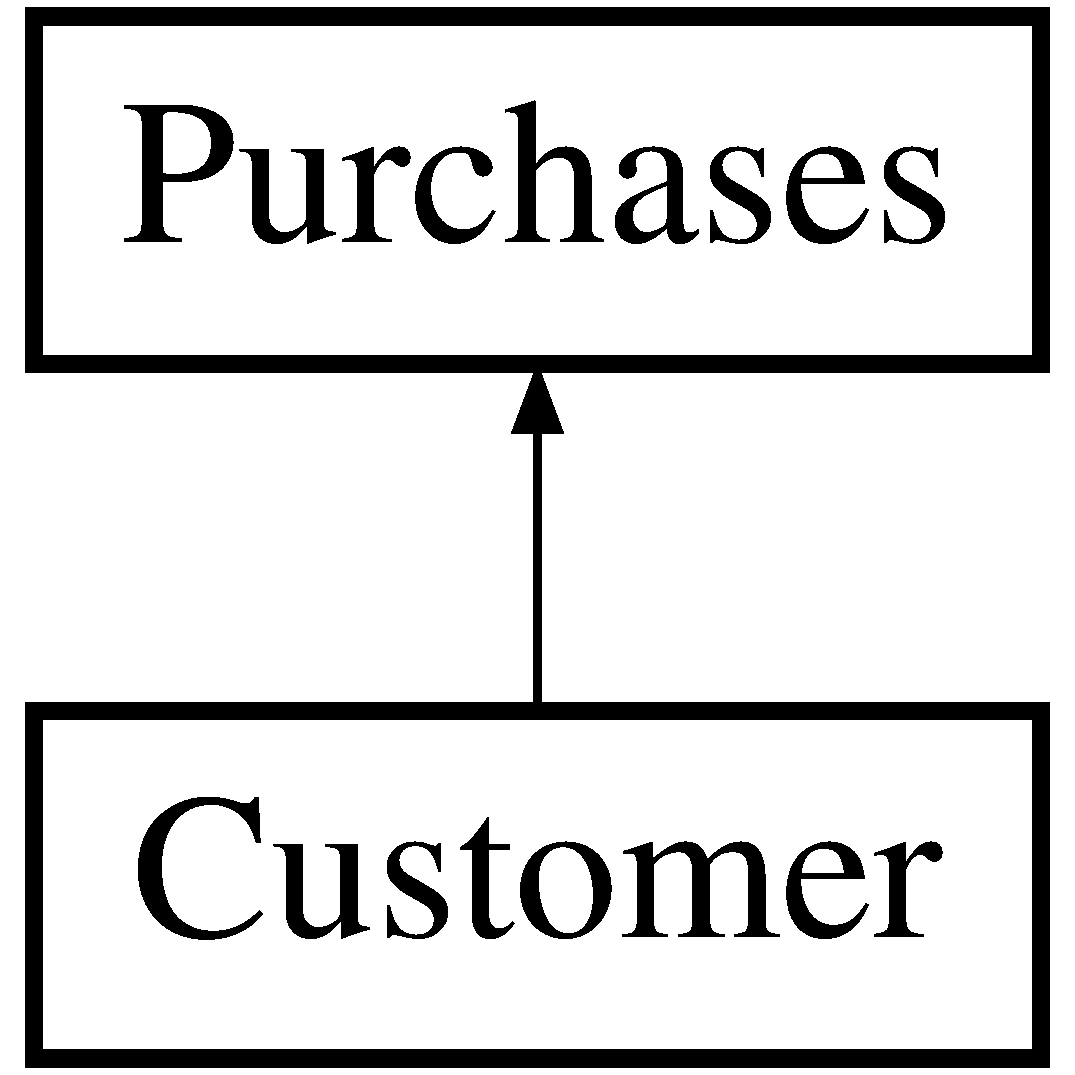
\includegraphics[height=2.000000cm]{class_customer}
\end{center}
\end{figure}
\subsection*{Public Member Functions}
\begin{DoxyCompactItemize}
\item 
\mbox{\Hypertarget{class_customer_aadd2561680381af9de9d3b9abdc54bb8}\label{class_customer_aadd2561680381af9de9d3b9abdc54bb8}} 
{\bfseries Customer} (Q\+String, Q\+String, Q\+String, Q\+String, Q\+String)
\item 
\mbox{\Hypertarget{class_customer_a551c3a7139081bc840501bc06c796e96}\label{class_customer_a551c3a7139081bc840501bc06c796e96}} 
{\bfseries Customer} (const \mbox{\hyperlink{class_customer}{Customer}} \&)
\item 
\mbox{\Hypertarget{class_customer_a65bcde40edff711f6a96847f4720e83e}\label{class_customer_a65bcde40edff711f6a96847f4720e83e}} 
virtual Q\+String {\bfseries get\+Customer\+Name} () const
\item 
\mbox{\Hypertarget{class_customer_a11886fba33594f13559f1ddd801cbe4c}\label{class_customer_a11886fba33594f13559f1ddd801cbe4c}} 
Q\+String {\bfseries get\+Customer\+Address} () const
\item 
\mbox{\Hypertarget{class_customer_a6847c0af28a15a96345205d8cd87bf8c}\label{class_customer_a6847c0af28a15a96345205d8cd87bf8c}} 
Q\+String {\bfseries get\+Customer\+Interest} () const
\item 
\mbox{\Hypertarget{class_customer_a60e7fe5a6c74f4aca05bdf836b1b1c5f}\label{class_customer_a60e7fe5a6c74f4aca05bdf836b1b1c5f}} 
Q\+String {\bfseries get\+Customer\+Rating} () const
\item 
\mbox{\Hypertarget{class_customer_ab74ea75c93b6ff556326d106f03237c8}\label{class_customer_ab74ea75c93b6ff556326d106f03237c8}} 
Q\+String {\bfseries get\+Customer\+Pamphlet} () const
\item 
\mbox{\Hypertarget{class_customer_a0c41e82116af74a6e49687b8f163a42e}\label{class_customer_a0c41e82116af74a6e49687b8f163a42e}} 
Q\+String {\bfseries get\+Seperated\+Address} () const
\end{DoxyCompactItemize}


The documentation for this class was generated from the following files\+:\begin{DoxyCompactItemize}
\item 
C\+:/\+Users/x\+Dead/\+One\+Drive/\+Desktop/\+Project2/customer.\+h\item 
C\+:/\+Users/x\+Dead/\+One\+Drive/\+Desktop/\+Project2/customer.\+cpp\end{DoxyCompactItemize}

\hypertarget{classdb_manager}{}\section{db\+Manager Class Reference}
\label{classdb_manager}\index{db\+Manager@{db\+Manager}}
\subsection*{Public Member Functions}
\begin{DoxyCompactItemize}
\item 
\mbox{\Hypertarget{classdb_manager_af72b6c137c35eb6b65f0a8082214e00a}\label{classdb_manager_af72b6c137c35eb6b65f0a8082214e00a}} 
bool {\bfseries is\+Open} () const
\item 
\mbox{\Hypertarget{classdb_manager_aa29c1c97044f4682191b27178fb0bc16}\label{classdb_manager_aa29c1c97044f4682191b27178fb0bc16}} 
{\bfseries db\+Manager} (const \mbox{\hyperlink{classdb_manager}{db\+Manager}} \&)=delete
\item 
\mbox{\Hypertarget{classdb_manager_aa10203218ffdde8956db859348dfc83f}\label{classdb_manager_aa10203218ffdde8956db859348dfc83f}} 
void {\bfseries operator=} (const \mbox{\hyperlink{classdb_manager}{db\+Manager}} \&)=delete
\item 
\mbox{\Hypertarget{classdb_manager_ae058bb3596b9f9d38c6b70957dfa1733}\label{classdb_manager_ae058bb3596b9f9d38c6b70957dfa1733}} 
bool {\bfseries customer\+Exists} (const \mbox{\hyperlink{class_customer}{Customer}} \&customer)
\item 
\mbox{\Hypertarget{classdb_manager_aea784d49fd19376a52b51ce6d3517936}\label{classdb_manager_aea784d49fd19376a52b51ce6d3517936}} 
bool {\bfseries add\+Customer} (const \mbox{\hyperlink{class_customer}{Customer}} \&new\+Customer)
\item 
\mbox{\Hypertarget{classdb_manager_a811b932e2ef4b109b6f38315fb20893f}\label{classdb_manager_a811b932e2ef4b109b6f38315fb20893f}} 
bool {\bfseries delete\+Customer} (const \mbox{\hyperlink{class_customer}{Customer}} \&customer)
\item 
\mbox{\Hypertarget{classdb_manager_af60293546bcf6e584f3b13867f544381}\label{classdb_manager_af60293546bcf6e584f3b13867f544381}} 
bool {\bfseries add\+Purchase} (const \mbox{\hyperlink{class_purchases}{Purchases}} \&new\+Purchase)
\end{DoxyCompactItemize}
\subsection*{Static Public Member Functions}
\begin{DoxyCompactItemize}
\item 
\mbox{\Hypertarget{classdb_manager_aca1b877120d3e7b7391d66973b3badb0}\label{classdb_manager_aca1b877120d3e7b7391d66973b3badb0}} 
static \mbox{\hyperlink{classdb_manager}{db\+Manager}} \& {\bfseries instance} ()
\end{DoxyCompactItemize}


The documentation for this class was generated from the following files\+:\begin{DoxyCompactItemize}
\item 
C\+:/\+Users/x\+Dead/\+One\+Drive/\+Desktop/\+Project2/dbmanager.\+h\item 
C\+:/\+Users/x\+Dead/\+One\+Drive/\+Desktop/\+Project2/dbmanager.\+cpp\end{DoxyCompactItemize}

\hypertarget{class_main_interface}{}\section{Main\+Interface Class Reference}
\label{class_main_interface}\index{Main\+Interface@{Main\+Interface}}
Inheritance diagram for Main\+Interface\+:\begin{figure}[H]
\begin{center}
\leavevmode
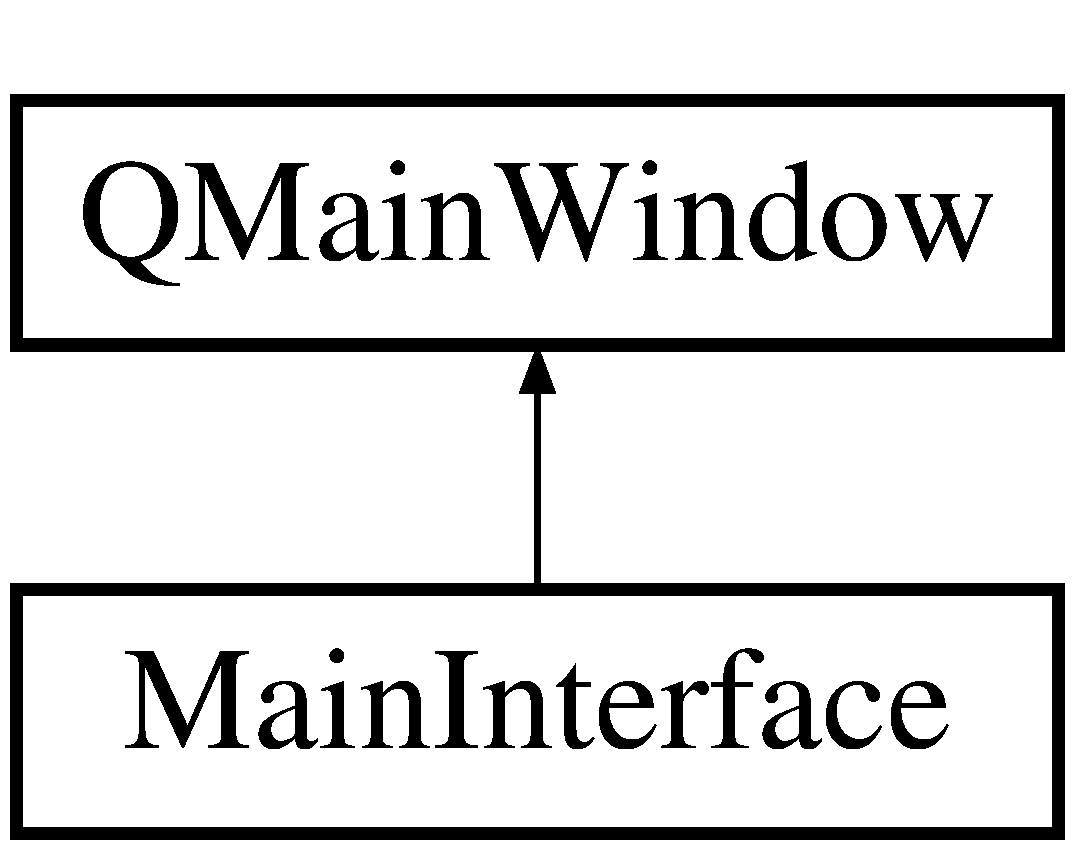
\includegraphics[height=2.000000cm]{class_main_interface}
\end{center}
\end{figure}
\subsection*{Public Member Functions}
\begin{DoxyCompactItemize}
\item 
\mbox{\Hypertarget{class_main_interface_a50ec59f9dc5489bbb18baae382dbc7ad}\label{class_main_interface_a50ec59f9dc5489bbb18baae382dbc7ad}} 
{\bfseries Main\+Interface} (Q\+Widget $\ast$parent=0)
\end{DoxyCompactItemize}


The documentation for this class was generated from the following files\+:\begin{DoxyCompactItemize}
\item 
C\+:/\+Users/x\+Dead/\+One\+Drive/\+Desktop/\+Project2/maininterface.\+h\item 
C\+:/\+Users/x\+Dead/\+One\+Drive/\+Desktop/\+Project2/maininterface.\+cpp\end{DoxyCompactItemize}

\hypertarget{class_ui_1_1_main_interface}{}\section{Ui\+:\+:Main\+Interface Class Reference}
\label{class_ui_1_1_main_interface}\index{Ui\+::\+Main\+Interface@{Ui\+::\+Main\+Interface}}
Inheritance diagram for Ui\+:\+:Main\+Interface\+:\begin{figure}[H]
\begin{center}
\leavevmode
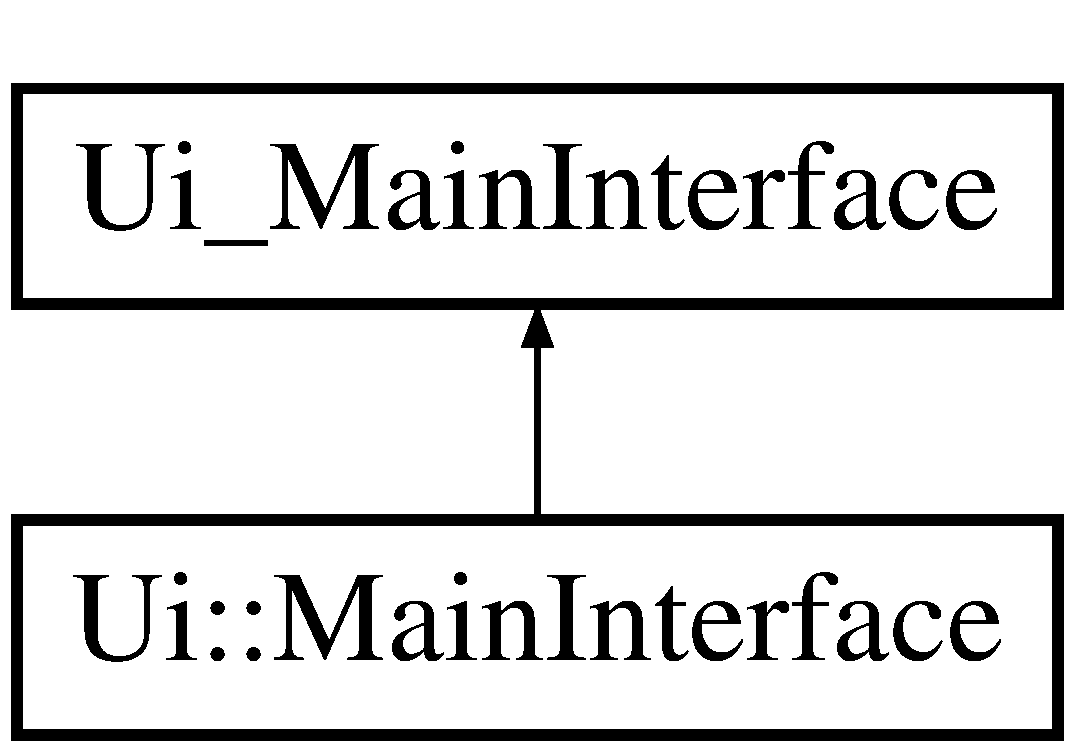
\includegraphics[height=2.000000cm]{class_ui_1_1_main_interface}
\end{center}
\end{figure}
\subsection*{Additional Inherited Members}


The documentation for this class was generated from the following file\+:\begin{DoxyCompactItemize}
\item 
C\+:/\+Users/x\+Dead/\+One\+Drive/\+Desktop/\+Project2/ui\+\_\+maininterface.\+h\end{DoxyCompactItemize}

\hypertarget{class_purchases}{}\section{Purchases Class Reference}
\label{class_purchases}\index{Purchases@{Purchases}}
Inheritance diagram for Purchases\+:\begin{figure}[H]
\begin{center}
\leavevmode
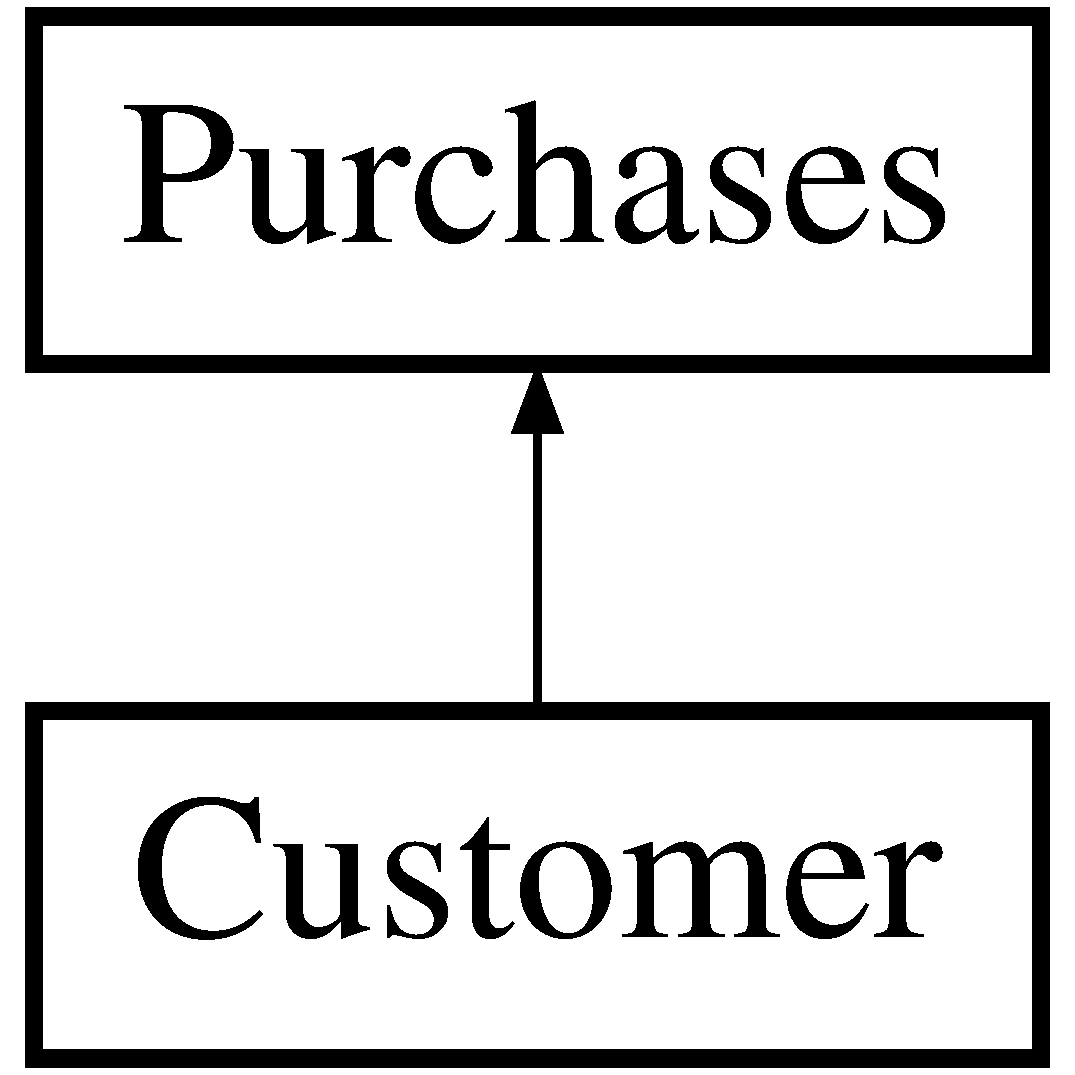
\includegraphics[height=2.000000cm]{class_purchases}
\end{center}
\end{figure}
\subsection*{Public Member Functions}
\begin{DoxyCompactItemize}
\item 
\mbox{\Hypertarget{class_purchases_ad44e2d8654199cec7d4fc2cbbc5f42a2}\label{class_purchases_ad44e2d8654199cec7d4fc2cbbc5f42a2}} 
{\bfseries Purchases} (Q\+String, int, int, int, double)
\item 
\mbox{\Hypertarget{class_purchases_ae42dffed0e0d98b7dc055b17137de9e6}\label{class_purchases_ae42dffed0e0d98b7dc055b17137de9e6}} 
Q\+String {\bfseries get\+Customer\+Name} () const
\item 
\mbox{\Hypertarget{class_purchases_ae6cbc35e6008368d4fb0d936f2d55b22}\label{class_purchases_ae6cbc35e6008368d4fb0d936f2d55b22}} 
int {\bfseries get\+Qty\+Silver} () const
\item 
\mbox{\Hypertarget{class_purchases_a73d8118537a82680f2d32baaf611c5e5}\label{class_purchases_a73d8118537a82680f2d32baaf611c5e5}} 
int {\bfseries get\+Qty\+Gold} () const
\item 
\mbox{\Hypertarget{class_purchases_a991e8a1000889b01ced9dd5f9b8d45ea}\label{class_purchases_a991e8a1000889b01ced9dd5f9b8d45ea}} 
int {\bfseries get\+Qty\+Plat} () const
\item 
\mbox{\Hypertarget{class_purchases_a2d3bcf94fecdfd384559d1861c7fbafe}\label{class_purchases_a2d3bcf94fecdfd384559d1861c7fbafe}} 
double {\bfseries get\+Sub\+Total} () const
\item 
\mbox{\Hypertarget{class_purchases_a92aabfb28dc5f836405295210ddcc55c}\label{class_purchases_a92aabfb28dc5f836405295210ddcc55c}} 
bool {\bfseries operator==} (const \mbox{\hyperlink{class_purchases}{Purchases}} \&)
\item 
\mbox{\Hypertarget{class_purchases_ada4bbbcc5530c402205f8c7eac1f3a6d}\label{class_purchases_ada4bbbcc5530c402205f8c7eac1f3a6d}} 
\mbox{\hyperlink{class_purchases}{Purchases}} {\bfseries operator-\/} (double)
\end{DoxyCompactItemize}


The documentation for this class was generated from the following files\+:\begin{DoxyCompactItemize}
\item 
C\+:/\+Users/x\+Dead/\+One\+Drive/\+Desktop/\+Project2/purchases.\+h\item 
C\+:/\+Users/x\+Dead/\+One\+Drive/\+Desktop/\+Project2/purchases.\+cpp\end{DoxyCompactItemize}

\hypertarget{structqt__meta__stringdata___main_interface__t}{}\section{qt\+\_\+meta\+\_\+stringdata\+\_\+\+Main\+Interface\+\_\+t Struct Reference}
\label{structqt__meta__stringdata___main_interface__t}\index{qt\+\_\+meta\+\_\+stringdata\+\_\+\+Main\+Interface\+\_\+t@{qt\+\_\+meta\+\_\+stringdata\+\_\+\+Main\+Interface\+\_\+t}}
\subsection*{Public Attributes}
\begin{DoxyCompactItemize}
\item 
\mbox{\Hypertarget{structqt__meta__stringdata___main_interface__t_a2cb4dc15ac28f74acbbe2fa87922b137}\label{structqt__meta__stringdata___main_interface__t_a2cb4dc15ac28f74acbbe2fa87922b137}} 
Q\+Byte\+Array\+Data {\bfseries data} \mbox{[}45\mbox{]}
\item 
\mbox{\Hypertarget{structqt__meta__stringdata___main_interface__t_a142f2cef1263a12def314232a89d49ed}\label{structqt__meta__stringdata___main_interface__t_a142f2cef1263a12def314232a89d49ed}} 
char {\bfseries stringdata0} \mbox{[}1095\mbox{]}
\end{DoxyCompactItemize}


The documentation for this struct was generated from the following file\+:\begin{DoxyCompactItemize}
\item 
C\+:/\+Users/x\+Dead/\+One\+Drive/\+Desktop/\+Project2/moc\+\_\+maininterface.\+cpp\end{DoxyCompactItemize}

\hypertarget{class_ui___main_interface}{}\section{Ui\+\_\+\+Main\+Interface Class Reference}
\label{class_ui___main_interface}\index{Ui\+\_\+\+Main\+Interface@{Ui\+\_\+\+Main\+Interface}}
Inheritance diagram for Ui\+\_\+\+Main\+Interface\+:\begin{figure}[H]
\begin{center}
\leavevmode
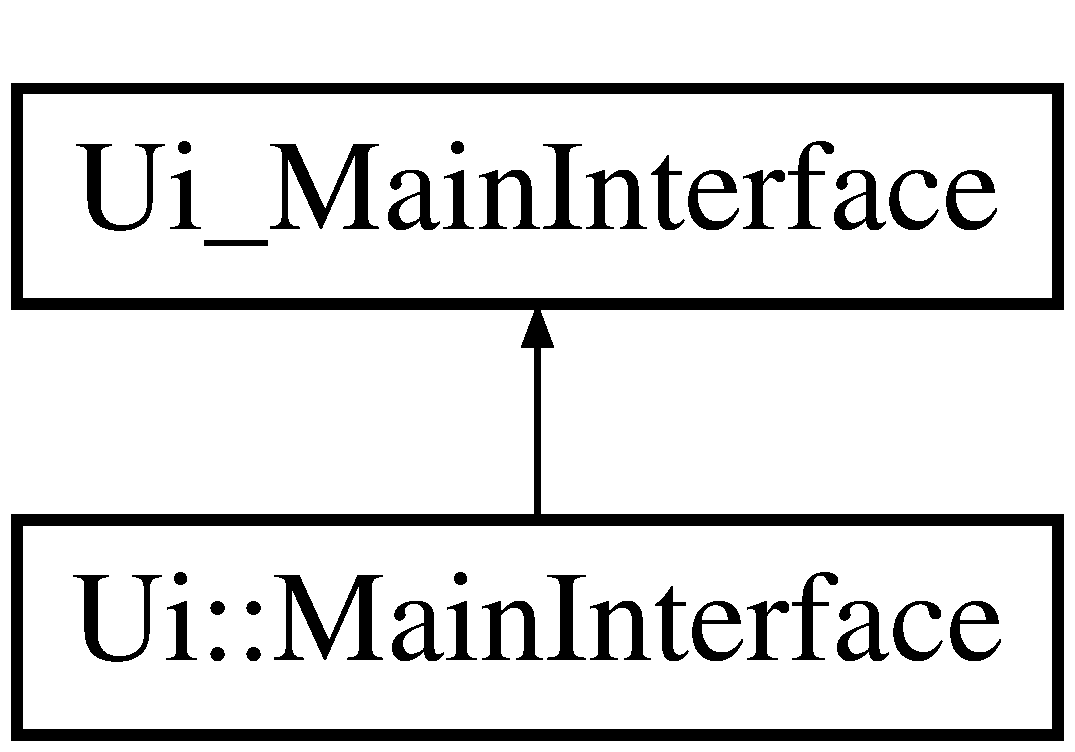
\includegraphics[height=2.000000cm]{class_ui___main_interface}
\end{center}
\end{figure}
\subsection*{Public Member Functions}
\begin{DoxyCompactItemize}
\item 
\mbox{\Hypertarget{class_ui___main_interface_aa8c09ad8ab5464eed7fe57eb946de29e}\label{class_ui___main_interface_aa8c09ad8ab5464eed7fe57eb946de29e}} 
void {\bfseries setup\+Ui} (Q\+Main\+Window $\ast$\mbox{\hyperlink{class_main_interface}{Main\+Interface}})
\item 
\mbox{\Hypertarget{class_ui___main_interface_a6650721ee7cf20dc3178cd34048985ad}\label{class_ui___main_interface_a6650721ee7cf20dc3178cd34048985ad}} 
void {\bfseries retranslate\+Ui} (Q\+Main\+Window $\ast$\mbox{\hyperlink{class_main_interface}{Main\+Interface}})
\end{DoxyCompactItemize}
\subsection*{Public Attributes}
\begin{DoxyCompactItemize}
\item 
\mbox{\Hypertarget{class_ui___main_interface_a9753323f5e89423f9e50fc86026a5a87}\label{class_ui___main_interface_a9753323f5e89423f9e50fc86026a5a87}} 
Q\+Widget $\ast$ {\bfseries central\+Widget}
\item 
\mbox{\Hypertarget{class_ui___main_interface_ad9215cced0a06764c9b64d9cbb408e77}\label{class_ui___main_interface_ad9215cced0a06764c9b64d9cbb408e77}} 
Q\+Tab\+Widget $\ast$ {\bfseries tab\+Widget}
\item 
\mbox{\Hypertarget{class_ui___main_interface_a7d1d9b5a7f8b97838edb7846d500ea29}\label{class_ui___main_interface_a7d1d9b5a7f8b97838edb7846d500ea29}} 
Q\+Widget $\ast$ {\bfseries Home}
\item 
\mbox{\Hypertarget{class_ui___main_interface_ad2608d8f8c8445323d1b1376f57c61f5}\label{class_ui___main_interface_ad2608d8f8c8445323d1b1376f57c61f5}} 
Q\+Stacked\+Widget $\ast$ {\bfseries Home\+Widget}
\item 
\mbox{\Hypertarget{class_ui___main_interface_a6e91e627071c9336ac1d68e9fe596d7f}\label{class_ui___main_interface_a6e91e627071c9336ac1d68e9fe596d7f}} 
Q\+Widget $\ast$ {\bfseries Home\+\_\+\+Page}
\item 
\mbox{\Hypertarget{class_ui___main_interface_a29dde10df8bede127debe430e9b7bc5f}\label{class_ui___main_interface_a29dde10df8bede127debe430e9b7bc5f}} 
Q\+Label $\ast$ {\bfseries Silver\+\_\+label}
\item 
\mbox{\Hypertarget{class_ui___main_interface_ad89d4f48646b6042117294ddfdd5a11d}\label{class_ui___main_interface_ad89d4f48646b6042117294ddfdd5a11d}} 
Q\+Label $\ast$ {\bfseries Gold\+\_\+label}
\item 
\mbox{\Hypertarget{class_ui___main_interface_a5eebb002df4f4f642d4d68ccf6235a31}\label{class_ui___main_interface_a5eebb002df4f4f642d4d68ccf6235a31}} 
Q\+Label $\ast$ {\bfseries Platinum\+\_\+label}
\item 
\mbox{\Hypertarget{class_ui___main_interface_a17828cf0c7428a22d80880aaa53e604b}\label{class_ui___main_interface_a17828cf0c7428a22d80880aaa53e604b}} 
Q\+Label $\ast$ {\bfseries label\+\_\+7}
\item 
\mbox{\Hypertarget{class_ui___main_interface_ae5f2d2bd3a04adec171b544588f663db}\label{class_ui___main_interface_ae5f2d2bd3a04adec171b544588f663db}} 
Q\+Label $\ast$ {\bfseries label\+\_\+4}
\item 
\mbox{\Hypertarget{class_ui___main_interface_a427eb344d75291cdd8197424e1e189cd}\label{class_ui___main_interface_a427eb344d75291cdd8197424e1e189cd}} 
Q\+Label $\ast$ {\bfseries label\+\_\+8}
\item 
\mbox{\Hypertarget{class_ui___main_interface_aac300015902ce8c2ef9fe6986895ffe9}\label{class_ui___main_interface_aac300015902ce8c2ef9fe6986895ffe9}} 
Q\+Label $\ast$ {\bfseries label\+\_\+12}
\item 
\mbox{\Hypertarget{class_ui___main_interface_aac9e6904c561668b0b5f149391835e0d}\label{class_ui___main_interface_aac9e6904c561668b0b5f149391835e0d}} 
Q\+Label $\ast$ {\bfseries label\+\_\+14}
\item 
\mbox{\Hypertarget{class_ui___main_interface_ac2d936975b902439391c83d4e791e5db}\label{class_ui___main_interface_ac2d936975b902439391c83d4e791e5db}} 
Q\+Label $\ast$ {\bfseries label\+\_\+50}
\item 
\mbox{\Hypertarget{class_ui___main_interface_aafc4d49f47e2aed5a96c5f56ddaeb8b3}\label{class_ui___main_interface_aafc4d49f47e2aed5a96c5f56ddaeb8b3}} 
Q\+Label $\ast$ {\bfseries label\+\_\+5}
\item 
\mbox{\Hypertarget{class_ui___main_interface_a43161ca804be8ea81802976d71aadbdc}\label{class_ui___main_interface_a43161ca804be8ea81802976d71aadbdc}} 
Q\+Label $\ast$ {\bfseries label\+\_\+13}
\item 
\mbox{\Hypertarget{class_ui___main_interface_a1d667f6b62002188746320eecb16cb25}\label{class_ui___main_interface_a1d667f6b62002188746320eecb16cb25}} 
Q\+Label $\ast$ {\bfseries label\+\_\+49}
\item 
\mbox{\Hypertarget{class_ui___main_interface_a529854c335596c2ff1e7b87ba379e81b}\label{class_ui___main_interface_a529854c335596c2ff1e7b87ba379e81b}} 
Q\+Label $\ast$ {\bfseries label\+\_\+9}
\item 
\mbox{\Hypertarget{class_ui___main_interface_ab9021cbd6de1bb074140998ba3d56f2a}\label{class_ui___main_interface_ab9021cbd6de1bb074140998ba3d56f2a}} 
Q\+Label $\ast$ {\bfseries label\+\_\+10}
\item 
\mbox{\Hypertarget{class_ui___main_interface_a96228a794543c807292b3080f01ed565}\label{class_ui___main_interface_a96228a794543c807292b3080f01ed565}} 
Q\+Label $\ast$ {\bfseries label\+\_\+48}
\item 
\mbox{\Hypertarget{class_ui___main_interface_a2af94b870050e1e15a56b9788d51a62f}\label{class_ui___main_interface_a2af94b870050e1e15a56b9788d51a62f}} 
Q\+Label $\ast$ {\bfseries label\+\_\+15}
\item 
\mbox{\Hypertarget{class_ui___main_interface_a0b3c936c383f71936b959b63b782f390}\label{class_ui___main_interface_a0b3c936c383f71936b959b63b782f390}} 
Q\+Label $\ast$ {\bfseries label\+\_\+17}
\item 
\mbox{\Hypertarget{class_ui___main_interface_a644cd83903fb42254a4d994475da529b}\label{class_ui___main_interface_a644cd83903fb42254a4d994475da529b}} 
Q\+Label $\ast$ {\bfseries label\+\_\+16}
\item 
\mbox{\Hypertarget{class_ui___main_interface_a140f4a085ea441d6f3d7885732af9f74}\label{class_ui___main_interface_a140f4a085ea441d6f3d7885732af9f74}} 
Q\+Label $\ast$ {\bfseries label\+\_\+18}
\item 
\mbox{\Hypertarget{class_ui___main_interface_a0c7ccfcd4614f6bbc4be524530472bb4}\label{class_ui___main_interface_a0c7ccfcd4614f6bbc4be524530472bb4}} 
Q\+Label $\ast$ {\bfseries label\+\_\+20}
\item 
\mbox{\Hypertarget{class_ui___main_interface_a4146e207803757b7afc5e51dfd32a4ee}\label{class_ui___main_interface_a4146e207803757b7afc5e51dfd32a4ee}} 
Q\+Label $\ast$ {\bfseries label\+\_\+19}
\item 
\mbox{\Hypertarget{class_ui___main_interface_aa1128c50ca2ab556b48f7ff07e6cc482}\label{class_ui___main_interface_aa1128c50ca2ab556b48f7ff07e6cc482}} 
Q\+Widget $\ast$ {\bfseries vertical\+Layout\+Widget\+\_\+2}
\item 
\mbox{\Hypertarget{class_ui___main_interface_a7dc3fbcf21868c8cb85d7069cf5e811a}\label{class_ui___main_interface_a7dc3fbcf21868c8cb85d7069cf5e811a}} 
Q\+V\+Box\+Layout $\ast$ {\bfseries vertical\+Layout\+\_\+2}
\item 
\mbox{\Hypertarget{class_ui___main_interface_a0a5f99023ff1024b4f5d05a8f2492a75}\label{class_ui___main_interface_a0a5f99023ff1024b4f5d05a8f2492a75}} 
Q\+Push\+Button $\ast$ {\bfseries buy\+Button}
\item 
\mbox{\Hypertarget{class_ui___main_interface_af99b8add3a141568d4599b3811e9fd5f}\label{class_ui___main_interface_af99b8add3a141568d4599b3811e9fd5f}} 
Q\+Push\+Button $\ast$ {\bfseries Get\+Pamphlet\+\_\+push\+Button}
\item 
\mbox{\Hypertarget{class_ui___main_interface_a8e5bf05ef05716b5a3c45a1925db8563}\label{class_ui___main_interface_a8e5bf05ef05716b5a3c45a1925db8563}} 
Q\+Frame $\ast$ {\bfseries frame}
\item 
\mbox{\Hypertarget{class_ui___main_interface_a9c38de536b87eb079409f565158ca1d1}\label{class_ui___main_interface_a9c38de536b87eb079409f565158ca1d1}} 
Q\+Push\+Button $\ast$ {\bfseries Silver\+Product\+Details}
\item 
\mbox{\Hypertarget{class_ui___main_interface_ad44f4048494d91cc7db9fec4394717f1}\label{class_ui___main_interface_ad44f4048494d91cc7db9fec4394717f1}} 
Q\+Frame $\ast$ {\bfseries frame\+\_\+2}
\item 
\mbox{\Hypertarget{class_ui___main_interface_a3bfa464ad244acd4f3ae4819343b4a71}\label{class_ui___main_interface_a3bfa464ad244acd4f3ae4819343b4a71}} 
Q\+Push\+Button $\ast$ {\bfseries Gold\+Product\+Details}
\item 
\mbox{\Hypertarget{class_ui___main_interface_a6bf76ea8a572ecff394d149f6c1df6e9}\label{class_ui___main_interface_a6bf76ea8a572ecff394d149f6c1df6e9}} 
Q\+Frame $\ast$ {\bfseries frame\+\_\+8}
\item 
\mbox{\Hypertarget{class_ui___main_interface_a5d2d344d0dcc33f5120764885f488384}\label{class_ui___main_interface_a5d2d344d0dcc33f5120764885f488384}} 
Q\+Push\+Button $\ast$ {\bfseries Platinum\+Product\+Details}
\item 
\mbox{\Hypertarget{class_ui___main_interface_af357dbf04624a34e5b4fb4f9ab9c140f}\label{class_ui___main_interface_af357dbf04624a34e5b4fb4f9ab9c140f}} 
Q\+Label $\ast$ {\bfseries label}
\item 
\mbox{\Hypertarget{class_ui___main_interface_a24d9cbd0574c30e68689006121c2a472}\label{class_ui___main_interface_a24d9cbd0574c30e68689006121c2a472}} 
Q\+Widget $\ast$ {\bfseries Platinum\+\_\+\+Info}
\item 
\mbox{\Hypertarget{class_ui___main_interface_aab18a4def2b0093b1012472827e5a4e7}\label{class_ui___main_interface_aab18a4def2b0093b1012472827e5a4e7}} 
Q\+Label $\ast$ {\bfseries Platinum\+\_\+label\+\_\+3}
\item 
\mbox{\Hypertarget{class_ui___main_interface_a3064b2d79729ffdd74344db732c13e50}\label{class_ui___main_interface_a3064b2d79729ffdd74344db732c13e50}} 
Q\+Push\+Button $\ast$ {\bfseries Platinum\+\_\+\+Back\+To\+Home}
\item 
\mbox{\Hypertarget{class_ui___main_interface_a3a3b7271d91a71844d775f2bd10c7321}\label{class_ui___main_interface_a3a3b7271d91a71844d775f2bd10c7321}} 
Q\+Text\+Edit $\ast$ {\bfseries Platinum\+\_\+text\+Edit}
\item 
\mbox{\Hypertarget{class_ui___main_interface_a3485d9472629371d675605a1df70f52f}\label{class_ui___main_interface_a3485d9472629371d675605a1df70f52f}} 
Q\+Widget $\ast$ {\bfseries Gold\+\_\+\+Info}
\item 
\mbox{\Hypertarget{class_ui___main_interface_a0603422af5909d5454a2004d7ab1f4fd}\label{class_ui___main_interface_a0603422af5909d5454a2004d7ab1f4fd}} 
Q\+Push\+Button $\ast$ {\bfseries Gold\+\_\+\+Back\+To\+Home\+\_\+2}
\item 
\mbox{\Hypertarget{class_ui___main_interface_aa6f04546d9d5e07f7f01f9d6acbe7ccc}\label{class_ui___main_interface_aa6f04546d9d5e07f7f01f9d6acbe7ccc}} 
Q\+Label $\ast$ {\bfseries Gold\+\_\+label\+\_\+2}
\item 
\mbox{\Hypertarget{class_ui___main_interface_ae8f3dccf6c4e4626fefad9cd1a043f5f}\label{class_ui___main_interface_ae8f3dccf6c4e4626fefad9cd1a043f5f}} 
Q\+Text\+Edit $\ast$ {\bfseries gold\+\_\+text\+Edit}
\item 
\mbox{\Hypertarget{class_ui___main_interface_a2b0e1c15cfec6695113c9f1546f9d51d}\label{class_ui___main_interface_a2b0e1c15cfec6695113c9f1546f9d51d}} 
Q\+Widget $\ast$ {\bfseries Silver\+\_\+\+Info}
\item 
\mbox{\Hypertarget{class_ui___main_interface_a0355d4bc7fc44ef32ae17e7db053c314}\label{class_ui___main_interface_a0355d4bc7fc44ef32ae17e7db053c314}} 
Q\+Label $\ast$ {\bfseries Silver\+\_\+label\+\_\+3}
\item 
\mbox{\Hypertarget{class_ui___main_interface_a7b9c62d24d04af8dea2f0c4a8b7e506a}\label{class_ui___main_interface_a7b9c62d24d04af8dea2f0c4a8b7e506a}} 
Q\+Push\+Button $\ast$ {\bfseries Silver\+\_\+\+Back\+To\+Home}
\item 
\mbox{\Hypertarget{class_ui___main_interface_a3c9ef61723f0ee292c101a925be92211}\label{class_ui___main_interface_a3c9ef61723f0ee292c101a925be92211}} 
Q\+Text\+Edit $\ast$ {\bfseries silver\+\_\+text\+Edit}
\item 
\mbox{\Hypertarget{class_ui___main_interface_aaab172a8fbb45cc9a5dbae6f1ba06efd}\label{class_ui___main_interface_aaab172a8fbb45cc9a5dbae6f1ba06efd}} 
Q\+Widget $\ast$ {\bfseries Pamphlet}
\item 
\mbox{\Hypertarget{class_ui___main_interface_ab9b7db6779d6dffbba827a11aa87716d}\label{class_ui___main_interface_ab9b7db6779d6dffbba827a11aa87716d}} 
Q\+Frame $\ast$ {\bfseries frame\+\_\+6}
\item 
\mbox{\Hypertarget{class_ui___main_interface_ababe490cd5df1aaf1b12928ee4e17b67}\label{class_ui___main_interface_ababe490cd5df1aaf1b12928ee4e17b67}} 
Q\+Widget $\ast$ {\bfseries grid\+Layout\+Widget\+\_\+10}
\item 
\mbox{\Hypertarget{class_ui___main_interface_aa4a9d419a2e41222fca9cbb354f09860}\label{class_ui___main_interface_aa4a9d419a2e41222fca9cbb354f09860}} 
Q\+Grid\+Layout $\ast$ {\bfseries grid\+Layout\+\_\+9}
\item 
\mbox{\Hypertarget{class_ui___main_interface_acd2d9b2284ef97314be5bd7f7de6813e}\label{class_ui___main_interface_acd2d9b2284ef97314be5bd7f7de6813e}} 
Q\+Line\+Edit $\ast$ {\bfseries line\+Edit\+\_\+27}
\item 
\mbox{\Hypertarget{class_ui___main_interface_a6d316b2d59a3d1cf84e1faa7ef3964fe}\label{class_ui___main_interface_a6d316b2d59a3d1cf84e1faa7ef3964fe}} 
Q\+Combo\+Box $\ast$ {\bfseries combo\+Box\+\_\+10}
\item 
\mbox{\Hypertarget{class_ui___main_interface_af72f7ed677be71095168ed30b27e3f80}\label{class_ui___main_interface_af72f7ed677be71095168ed30b27e3f80}} 
Q\+Combo\+Box $\ast$ {\bfseries combo\+Box\+\_\+11}
\item 
\mbox{\Hypertarget{class_ui___main_interface_a158400d6799c898bc5c07460d9ebd55e}\label{class_ui___main_interface_a158400d6799c898bc5c07460d9ebd55e}} 
Q\+Line\+Edit $\ast$ {\bfseries line\+Edit\+\_\+28}
\item 
\mbox{\Hypertarget{class_ui___main_interface_a0a2a998738553381b8350257800b0fa3}\label{class_ui___main_interface_a0a2a998738553381b8350257800b0fa3}} 
Q\+Line\+Edit $\ast$ {\bfseries line\+Edit\+\_\+29}
\item 
\mbox{\Hypertarget{class_ui___main_interface_ac8ee091f48743a390dc3c2e799dea510}\label{class_ui___main_interface_ac8ee091f48743a390dc3c2e799dea510}} 
Q\+Line\+Edit $\ast$ {\bfseries line\+Edit\+\_\+30}
\item 
\mbox{\Hypertarget{class_ui___main_interface_a975eb68fdc843b59db1d9ec4774b717e}\label{class_ui___main_interface_a975eb68fdc843b59db1d9ec4774b717e}} 
Q\+Line\+Edit $\ast$ {\bfseries line\+Edit\+\_\+31}
\item 
\mbox{\Hypertarget{class_ui___main_interface_af5065d9c4baa517311b373c5e5b6e782}\label{class_ui___main_interface_af5065d9c4baa517311b373c5e5b6e782}} 
Q\+Line\+Edit $\ast$ {\bfseries line\+Edit\+\_\+32}
\item 
\mbox{\Hypertarget{class_ui___main_interface_af4a48b54e7b4d2167df262e9878c4995}\label{class_ui___main_interface_af4a48b54e7b4d2167df262e9878c4995}} 
Q\+Widget $\ast$ {\bfseries grid\+Layout\+Widget\+\_\+11}
\item 
\mbox{\Hypertarget{class_ui___main_interface_a019e6a76bd75a6b48e052b8047e60bae}\label{class_ui___main_interface_a019e6a76bd75a6b48e052b8047e60bae}} 
Q\+Grid\+Layout $\ast$ {\bfseries grid\+Layout\+\_\+10}
\item 
\mbox{\Hypertarget{class_ui___main_interface_acdcb161b0e71ec82f086b38742be12d0}\label{class_ui___main_interface_acdcb161b0e71ec82f086b38742be12d0}} 
Q\+Line\+Edit $\ast$ {\bfseries city\+\_\+line\+Edit\+\_\+2}
\item 
\mbox{\Hypertarget{class_ui___main_interface_a13fd73b06440eb9089c2ebf56cdb762d}\label{class_ui___main_interface_a13fd73b06440eb9089c2ebf56cdb762d}} 
Q\+Line\+Edit $\ast$ {\bfseries zip\+\_\+line\+Edit\+\_\+2}
\item 
\mbox{\Hypertarget{class_ui___main_interface_a312d0f9520243b4b5d79712a15ec22b9}\label{class_ui___main_interface_a312d0f9520243b4b5d79712a15ec22b9}} 
Q\+Combo\+Box $\ast$ {\bfseries state\+\_\+combo\+Box\+\_\+2}
\item 
\mbox{\Hypertarget{class_ui___main_interface_a2083eb95d078391cdb943c352c968b8f}\label{class_ui___main_interface_a2083eb95d078391cdb943c352c968b8f}} 
Q\+Combo\+Box $\ast$ {\bfseries country\+\_\+combo\+Box\+\_\+2}
\item 
\mbox{\Hypertarget{class_ui___main_interface_a31d3fee2b24b744e4b4207f10498da05}\label{class_ui___main_interface_a31d3fee2b24b744e4b4207f10498da05}} 
Q\+Line\+Edit $\ast$ {\bfseries address\+\_\+line\+Edit\+\_\+2}
\item 
\mbox{\Hypertarget{class_ui___main_interface_aefe9fd30d37a1e343b57146346483763}\label{class_ui___main_interface_aefe9fd30d37a1e343b57146346483763}} 
Q\+Line\+Edit $\ast$ {\bfseries first\+Name\+\_\+line\+Edit\+\_\+2}
\item 
\mbox{\Hypertarget{class_ui___main_interface_a5a497955c740dddb7d3f1c7276ee05e1}\label{class_ui___main_interface_a5a497955c740dddb7d3f1c7276ee05e1}} 
Q\+Label $\ast$ {\bfseries bill\+Address\+\_\+label\+\_\+2}
\item 
\mbox{\Hypertarget{class_ui___main_interface_a5777a5ff6d2d2890d5b552683e5639db}\label{class_ui___main_interface_a5777a5ff6d2d2890d5b552683e5639db}} 
Q\+Widget $\ast$ {\bfseries vertical\+Layout\+Widget\+\_\+7}
\item 
\mbox{\Hypertarget{class_ui___main_interface_af0420f1e6fc50e8ed78e2e55f1b28070}\label{class_ui___main_interface_af0420f1e6fc50e8ed78e2e55f1b28070}} 
Q\+V\+Box\+Layout $\ast$ {\bfseries vertical\+Layout\+\_\+7}
\item 
\mbox{\Hypertarget{class_ui___main_interface_a7fcff6ec6c40bab2f87f43f271c71fff}\label{class_ui___main_interface_a7fcff6ec6c40bab2f87f43f271c71fff}} 
Q\+Push\+Button $\ast$ {\bfseries pamplet\+\_\+button}
\item 
\mbox{\Hypertarget{class_ui___main_interface_a48b301863e1e7f675522f73766fb31d6}\label{class_ui___main_interface_a48b301863e1e7f675522f73766fb31d6}} 
Q\+Push\+Button $\ast$ {\bfseries Pamplet\+\_\+\+Back\+To\+Home}
\item 
\mbox{\Hypertarget{class_ui___main_interface_ad9fd2aee9a364e456dcca21e1838fb57}\label{class_ui___main_interface_ad9fd2aee9a364e456dcca21e1838fb57}} 
Q\+Label $\ast$ {\bfseries pamplet\+Status}
\item 
\mbox{\Hypertarget{class_ui___main_interface_afded1d2f708d9c22565968a28fd603e0}\label{class_ui___main_interface_afded1d2f708d9c22565968a28fd603e0}} 
Q\+Label $\ast$ {\bfseries Company\+\_\+label\+\_\+4}
\item 
\mbox{\Hypertarget{class_ui___main_interface_a055865caf3714b942f9358d48498ee6a}\label{class_ui___main_interface_a055865caf3714b942f9358d48498ee6a}} 
Q\+Widget $\ast$ {\bfseries About}
\item 
\mbox{\Hypertarget{class_ui___main_interface_a2e57fe528e63ff52fd8cebc0fe389e40}\label{class_ui___main_interface_a2e57fe528e63ff52fd8cebc0fe389e40}} 
Q\+Label $\ast$ {\bfseries Company\+\_\+label\+\_\+5}
\item 
\mbox{\Hypertarget{class_ui___main_interface_a0201064b550089c7454a2413bd376e3c}\label{class_ui___main_interface_a0201064b550089c7454a2413bd376e3c}} 
Q\+Label $\ast$ {\bfseries about\+Us\+\_\+label}
\item 
\mbox{\Hypertarget{class_ui___main_interface_ac1d1502a3b59b9fdaa638bfafb5d59e5}\label{class_ui___main_interface_ac1d1502a3b59b9fdaa638bfafb5d59e5}} 
Q\+Text\+Edit $\ast$ {\bfseries about\+Us\+\_\+text\+Edit}
\item 
\mbox{\Hypertarget{class_ui___main_interface_afdfaa513cd64cdee59c2704af1da2420}\label{class_ui___main_interface_afdfaa513cd64cdee59c2704af1da2420}} 
Q\+Widget $\ast$ {\bfseries Reviews}
\item 
\mbox{\Hypertarget{class_ui___main_interface_a5533120bb835a71ca1a2d71bc88cb600}\label{class_ui___main_interface_a5533120bb835a71ca1a2d71bc88cb600}} 
Q\+Stacked\+Widget $\ast$ {\bfseries Review\+\_\+\+Page}
\item 
\mbox{\Hypertarget{class_ui___main_interface_a18ab65b6b6aff88b9f54f795aea95ebf}\label{class_ui___main_interface_a18ab65b6b6aff88b9f54f795aea95ebf}} 
Q\+Widget $\ast$ {\bfseries Show\+Reviews}
\item 
\mbox{\Hypertarget{class_ui___main_interface_af90b69e8ac42601b5b1530edf447a42e}\label{class_ui___main_interface_af90b69e8ac42601b5b1530edf447a42e}} 
Q\+Push\+Button $\ast$ {\bfseries Write\+Review\+Button}
\item 
\mbox{\Hypertarget{class_ui___main_interface_a70e5856333ab3eaa82a179da9d663292}\label{class_ui___main_interface_a70e5856333ab3eaa82a179da9d663292}} 
Q\+Table\+View $\ast$ {\bfseries table\+Review}
\item 
\mbox{\Hypertarget{class_ui___main_interface_a401693a322b24f6eeb74678ff2dcd8c2}\label{class_ui___main_interface_a401693a322b24f6eeb74678ff2dcd8c2}} 
Q\+Widget $\ast$ {\bfseries Write\+Review}
\item 
\mbox{\Hypertarget{class_ui___main_interface_a0246913c01ba050a91bd30cbddd20615}\label{class_ui___main_interface_a0246913c01ba050a91bd30cbddd20615}} 
Q\+Widget $\ast$ {\bfseries form\+Layout\+Widget}
\item 
\mbox{\Hypertarget{class_ui___main_interface_a19b162b6c02ee0574d0a0430e7c138d0}\label{class_ui___main_interface_a19b162b6c02ee0574d0a0430e7c138d0}} 
Q\+Form\+Layout $\ast$ {\bfseries form\+Layout}
\item 
\mbox{\Hypertarget{class_ui___main_interface_a5343dccb02a419f08e5e6d25d2eb0219}\label{class_ui___main_interface_a5343dccb02a419f08e5e6d25d2eb0219}} 
Q\+Label $\ast$ {\bfseries label\+\_\+22}
\item 
\mbox{\Hypertarget{class_ui___main_interface_adb2b0f33131fd158c6c7a35ef7496f4a}\label{class_ui___main_interface_adb2b0f33131fd158c6c7a35ef7496f4a}} 
Q\+Combo\+Box $\ast$ {\bfseries product\+\_\+combo\+Box}
\item 
\mbox{\Hypertarget{class_ui___main_interface_a7529cff13edddc602d7ddfcad6f32f67}\label{class_ui___main_interface_a7529cff13edddc602d7ddfcad6f32f67}} 
Q\+Label $\ast$ {\bfseries label\+\_\+23}
\item 
\mbox{\Hypertarget{class_ui___main_interface_ada2d6b3615df100d3bf515417c3873d0}\label{class_ui___main_interface_ada2d6b3615df100d3bf515417c3873d0}} 
Q\+Spin\+Box $\ast$ {\bfseries rate\+\_\+spin\+Box}
\item 
\mbox{\Hypertarget{class_ui___main_interface_a50c9109664398428db13e3e76938f416}\label{class_ui___main_interface_a50c9109664398428db13e3e76938f416}} 
Q\+Label $\ast$ {\bfseries label\+\_\+25}
\item 
\mbox{\Hypertarget{class_ui___main_interface_a68074e1821624d227f504c48a4f1d5be}\label{class_ui___main_interface_a68074e1821624d227f504c48a4f1d5be}} 
Q\+Line\+Edit $\ast$ {\bfseries name\+\_\+line\+Edit}
\item 
\mbox{\Hypertarget{class_ui___main_interface_aca616c99e6a59051107fd3c2ca62ae85}\label{class_ui___main_interface_aca616c99e6a59051107fd3c2ca62ae85}} 
Q\+Label $\ast$ {\bfseries label\+\_\+24}
\item 
\mbox{\Hypertarget{class_ui___main_interface_aedb60444690ee558e254015f599f0a98}\label{class_ui___main_interface_aedb60444690ee558e254015f599f0a98}} 
Q\+Text\+Edit $\ast$ {\bfseries review\+\_\+text\+Edit}
\item 
\mbox{\Hypertarget{class_ui___main_interface_ae0ee821ad28e2220083149311991fb5a}\label{class_ui___main_interface_ae0ee821ad28e2220083149311991fb5a}} 
Q\+Label $\ast$ {\bfseries review\+Status}
\item 
\mbox{\Hypertarget{class_ui___main_interface_a875a7f8caf58f84eca24caa15269d1ed}\label{class_ui___main_interface_a875a7f8caf58f84eca24caa15269d1ed}} 
Q\+Dialog\+Button\+Box $\ast$ {\bfseries button\+Box}
\item 
\mbox{\Hypertarget{class_ui___main_interface_a5a3ec43336f42f87dc2c6838cc9318e2}\label{class_ui___main_interface_a5a3ec43336f42f87dc2c6838cc9318e2}} 
Q\+Label $\ast$ {\bfseries Company\+\_\+label\+\_\+6}
\item 
\mbox{\Hypertarget{class_ui___main_interface_a9d9489cf494d219a349bbd97318fa231}\label{class_ui___main_interface_a9d9489cf494d219a349bbd97318fa231}} 
Q\+Widget $\ast$ {\bfseries Purchase}
\item 
\mbox{\Hypertarget{class_ui___main_interface_a07c34090f085f4a3ea5f21ace670e7ce}\label{class_ui___main_interface_a07c34090f085f4a3ea5f21ace670e7ce}} 
Q\+Stacked\+Widget $\ast$ {\bfseries Payment\+Information}
\item 
\mbox{\Hypertarget{class_ui___main_interface_afc752c1c7740db1eabe928a815bd6f36}\label{class_ui___main_interface_afc752c1c7740db1eabe928a815bd6f36}} 
Q\+Widget $\ast$ {\bfseries Choosing\+Product}
\item 
\mbox{\Hypertarget{class_ui___main_interface_ae5f28b77b792d17fc82adc6161321bb9}\label{class_ui___main_interface_ae5f28b77b792d17fc82adc6161321bb9}} 
Q\+Frame $\ast$ {\bfseries Frame1}
\item 
\mbox{\Hypertarget{class_ui___main_interface_ac3a7fa2eeacc6656f4990978aa4ac690}\label{class_ui___main_interface_ac3a7fa2eeacc6656f4990978aa4ac690}} 
Q\+Widget $\ast$ {\bfseries grid\+Layout\+Widget\+\_\+2}
\item 
\mbox{\Hypertarget{class_ui___main_interface_acccc387b767410c2b1683362c5b93945}\label{class_ui___main_interface_acccc387b767410c2b1683362c5b93945}} 
Q\+Grid\+Layout $\ast$ {\bfseries What\+To\+Purchase}
\item 
\mbox{\Hypertarget{class_ui___main_interface_a989ff142e0be2343620f3d14206fc137}\label{class_ui___main_interface_a989ff142e0be2343620f3d14206fc137}} 
Q\+Label $\ast$ {\bfseries gold\+Description1}
\item 
\mbox{\Hypertarget{class_ui___main_interface_a4496966db42a95132460432c5bee28b8}\label{class_ui___main_interface_a4496966db42a95132460432c5bee28b8}} 
Q\+Label $\ast$ {\bfseries Platinum\+Description2}
\item 
\mbox{\Hypertarget{class_ui___main_interface_ac87897582aeea22dbb062bbe8e5bd8fb}\label{class_ui___main_interface_ac87897582aeea22dbb062bbe8e5bd8fb}} 
Q\+Label $\ast$ {\bfseries Silver\+\_\+label\+\_\+2}
\item 
\mbox{\Hypertarget{class_ui___main_interface_a84d699cde9d53744b4df4b5f4ca9a339}\label{class_ui___main_interface_a84d699cde9d53744b4df4b5f4ca9a339}} 
Q\+Label $\ast$ {\bfseries product\+\_\+label}
\item 
\mbox{\Hypertarget{class_ui___main_interface_a0e9d507b3a0d8e8e2c656bbcf1d98d41}\label{class_ui___main_interface_a0e9d507b3a0d8e8e2c656bbcf1d98d41}} 
Q\+Label $\ast$ {\bfseries Platinum\+Description1}
\item 
\mbox{\Hypertarget{class_ui___main_interface_aa6bb4be4d950d22160565708cb88f601}\label{class_ui___main_interface_aa6bb4be4d950d22160565708cb88f601}} 
Q\+Label $\ast$ {\bfseries silver\+Price\+\_\+label}
\item 
\mbox{\Hypertarget{class_ui___main_interface_aa86277c1c5ed5a2e08765cd8dd2bf74e}\label{class_ui___main_interface_aa86277c1c5ed5a2e08765cd8dd2bf74e}} 
Q\+Label $\ast$ {\bfseries Platinum\+Description3}
\item 
\mbox{\Hypertarget{class_ui___main_interface_ade3fe509c144d4489c871731384785c2}\label{class_ui___main_interface_ade3fe509c144d4489c871731384785c2}} 
Q\+Spin\+Box $\ast$ {\bfseries platinum\+\_\+spin\+Box}
\item 
\mbox{\Hypertarget{class_ui___main_interface_a68283a6267f350632b1d7cab2b1b455c}\label{class_ui___main_interface_a68283a6267f350632b1d7cab2b1b455c}} 
Q\+Label $\ast$ {\bfseries price\+\_\+label}
\item 
\mbox{\Hypertarget{class_ui___main_interface_aa4562a967b1e99e2c9cddf5b30d5dda3}\label{class_ui___main_interface_aa4562a967b1e99e2c9cddf5b30d5dda3}} 
Q\+Label $\ast$ {\bfseries Platinum\+\_\+label\+\_\+2}
\item 
\mbox{\Hypertarget{class_ui___main_interface_a5a963f8e1958af63085d6174f524d579}\label{class_ui___main_interface_a5a963f8e1958af63085d6174f524d579}} 
Q\+Label $\ast$ {\bfseries sliver\+Description2}
\item 
\mbox{\Hypertarget{class_ui___main_interface_a80b2e1dcaf433ac97709957da850e014}\label{class_ui___main_interface_a80b2e1dcaf433ac97709957da850e014}} 
Q\+Label $\ast$ {\bfseries gold\+\_\+label}
\item 
\mbox{\Hypertarget{class_ui___main_interface_aa19579e80589528068088f80d5eafb18}\label{class_ui___main_interface_aa19579e80589528068088f80d5eafb18}} 
Q\+Spin\+Box $\ast$ {\bfseries gold\+\_\+spin\+Box}
\item 
\mbox{\Hypertarget{class_ui___main_interface_ab71ae44d2ff6ec8ef409fcdaa6882987}\label{class_ui___main_interface_ab71ae44d2ff6ec8ef409fcdaa6882987}} 
Q\+Label $\ast$ {\bfseries sliver\+Description3}
\item 
\mbox{\Hypertarget{class_ui___main_interface_adfe4e38f7e53c43b2c8f8c249eeac9a4}\label{class_ui___main_interface_adfe4e38f7e53c43b2c8f8c249eeac9a4}} 
Q\+Spin\+Box $\ast$ {\bfseries silver\+\_\+spin\+Box}
\item 
\mbox{\Hypertarget{class_ui___main_interface_a19bf2cfa3dc44128c9a3233222ea0659}\label{class_ui___main_interface_a19bf2cfa3dc44128c9a3233222ea0659}} 
Q\+Label $\ast$ {\bfseries qty\+\_\+label}
\item 
\mbox{\Hypertarget{class_ui___main_interface_ab17744defda2ff748743966a4a72a6ab}\label{class_ui___main_interface_ab17744defda2ff748743966a4a72a6ab}} 
Q\+Label $\ast$ {\bfseries sliver\+Description1}
\item 
\mbox{\Hypertarget{class_ui___main_interface_a15f126377974607d68306df72976f675}\label{class_ui___main_interface_a15f126377974607d68306df72976f675}} 
Q\+Label $\ast$ {\bfseries gold\+Description2}
\item 
\mbox{\Hypertarget{class_ui___main_interface_add2b107e59fd5436a79487b36fde7144}\label{class_ui___main_interface_add2b107e59fd5436a79487b36fde7144}} 
Q\+Label $\ast$ {\bfseries Platinum\+Price\+\_\+label\+\_\+2}
\item 
\mbox{\Hypertarget{class_ui___main_interface_a74592df3a5ceef433576695d3b375643}\label{class_ui___main_interface_a74592df3a5ceef433576695d3b375643}} 
Q\+Label $\ast$ {\bfseries gold\+Description3}
\item 
\mbox{\Hypertarget{class_ui___main_interface_ac19afc2b820524f42aa240ea75c4f0c4}\label{class_ui___main_interface_ac19afc2b820524f42aa240ea75c4f0c4}} 
Q\+Label $\ast$ {\bfseries Gold\+Price\+\_\+label}
\item 
\mbox{\Hypertarget{class_ui___main_interface_a312f361b0632d625573bc075151280b0}\label{class_ui___main_interface_a312f361b0632d625573bc075151280b0}} 
Q\+Push\+Button $\ast$ {\bfseries Buy\+Now\+Button}
\item 
\mbox{\Hypertarget{class_ui___main_interface_a0241dfaebc9322708c433a12f6dcc4e2}\label{class_ui___main_interface_a0241dfaebc9322708c433a12f6dcc4e2}} 
Q\+Widget $\ast$ {\bfseries Confirmation}
\item 
\mbox{\Hypertarget{class_ui___main_interface_ac265b807f8e15d7993e3711746d41b46}\label{class_ui___main_interface_ac265b807f8e15d7993e3711746d41b46}} 
Q\+Push\+Button $\ast$ {\bfseries Back\+Button}
\item 
\mbox{\Hypertarget{class_ui___main_interface_a36f70384a2034a71a46c94376b09244f}\label{class_ui___main_interface_a36f70384a2034a71a46c94376b09244f}} 
Q\+Frame $\ast$ {\bfseries frame\+\_\+7}
\item 
\mbox{\Hypertarget{class_ui___main_interface_a5b3688ea455a6e343fecfb7f830d2772}\label{class_ui___main_interface_a5b3688ea455a6e343fecfb7f830d2772}} 
Q\+Widget $\ast$ {\bfseries grid\+Layout\+Widget\+\_\+17}
\item 
\mbox{\Hypertarget{class_ui___main_interface_a4dae6b27d4ad1aac41d1c6395efcec61}\label{class_ui___main_interface_a4dae6b27d4ad1aac41d1c6395efcec61}} 
Q\+Grid\+Layout $\ast$ {\bfseries grid\+Layout\+\_\+16}
\item 
\mbox{\Hypertarget{class_ui___main_interface_a78573fdb53bf331284b506c13307c5e7}\label{class_ui___main_interface_a78573fdb53bf331284b506c13307c5e7}} 
Q\+Label $\ast$ {\bfseries gold\+Qty\+Purchased}
\item 
\mbox{\Hypertarget{class_ui___main_interface_a45bac29818b31f8a9335cc3e7a518763}\label{class_ui___main_interface_a45bac29818b31f8a9335cc3e7a518763}} 
Q\+Label $\ast$ {\bfseries label\+\_\+56}
\item 
\mbox{\Hypertarget{class_ui___main_interface_a9288d139ecb5afdf5932e7e51b61c6c6}\label{class_ui___main_interface_a9288d139ecb5afdf5932e7e51b61c6c6}} 
Q\+Label $\ast$ {\bfseries label\+\_\+59}
\item 
\mbox{\Hypertarget{class_ui___main_interface_af618c08c21ea2ba71b11e96dbaaaba78}\label{class_ui___main_interface_af618c08c21ea2ba71b11e96dbaaaba78}} 
Q\+Label $\ast$ {\bfseries total\+Amount\+\_\+2}
\item 
\mbox{\Hypertarget{class_ui___main_interface_ad0a4ee9cb4b5b801c8c684d51d9cc058}\label{class_ui___main_interface_ad0a4ee9cb4b5b801c8c684d51d9cc058}} 
Q\+Label $\ast$ {\bfseries sales\+Tax\+\_\+2}
\item 
\mbox{\Hypertarget{class_ui___main_interface_af1d73d104ae3189c856bb101ff916d0c}\label{class_ui___main_interface_af1d73d104ae3189c856bb101ff916d0c}} 
Q\+Label $\ast$ {\bfseries label\+\_\+61}
\item 
\mbox{\Hypertarget{class_ui___main_interface_a4f9b3dd517cbd50a88ae66a9fee83a23}\label{class_ui___main_interface_a4f9b3dd517cbd50a88ae66a9fee83a23}} 
Q\+Label $\ast$ {\bfseries label\+\_\+60}
\item 
\mbox{\Hypertarget{class_ui___main_interface_a039615bb6aace8cc8f34295cebe9c6b2}\label{class_ui___main_interface_a039615bb6aace8cc8f34295cebe9c6b2}} 
Q\+Label $\ast$ {\bfseries label\+\_\+58}
\item 
\mbox{\Hypertarget{class_ui___main_interface_a8fb6a2574ceb7f6e2f956504d2858ced}\label{class_ui___main_interface_a8fb6a2574ceb7f6e2f956504d2858ced}} 
Q\+Label $\ast$ {\bfseries label\+\_\+57}
\item 
\mbox{\Hypertarget{class_ui___main_interface_a8c79116407f6f505d69cc59db79fbf30}\label{class_ui___main_interface_a8c79116407f6f505d69cc59db79fbf30}} 
Q\+Label $\ast$ {\bfseries subtotal\+\_\+2}
\item 
\mbox{\Hypertarget{class_ui___main_interface_a199f867032cf9b913a264f4757d9733d}\label{class_ui___main_interface_a199f867032cf9b913a264f4757d9733d}} 
Q\+Label $\ast$ {\bfseries label\+\_\+54}
\item 
\mbox{\Hypertarget{class_ui___main_interface_a8759e885ae98b1e6741bd3716c41fc1f}\label{class_ui___main_interface_a8759e885ae98b1e6741bd3716c41fc1f}} 
Q\+Label $\ast$ {\bfseries Platinum\+Qty\+Purchased}
\item 
\mbox{\Hypertarget{class_ui___main_interface_acf41286abc01acb32ab90aabea91bab2}\label{class_ui___main_interface_acf41286abc01acb32ab90aabea91bab2}} 
Q\+Label $\ast$ {\bfseries label\+\_\+62}
\item 
\mbox{\Hypertarget{class_ui___main_interface_a45eacbc9da65f00456b640eae37d274f}\label{class_ui___main_interface_a45eacbc9da65f00456b640eae37d274f}} 
Q\+Label $\ast$ {\bfseries silver\+Qty\+Purchased}
\item 
\mbox{\Hypertarget{class_ui___main_interface_a506517d5bf9b4df8dedcf4265aa1b324}\label{class_ui___main_interface_a506517d5bf9b4df8dedcf4265aa1b324}} 
Q\+Spacer\+Item $\ast$ {\bfseries vertical\+Spacer\+\_\+11}
\item 
\mbox{\Hypertarget{class_ui___main_interface_aa9b01fe3707d975c0d31ff235af292c7}\label{class_ui___main_interface_aa9b01fe3707d975c0d31ff235af292c7}} 
Q\+Label $\ast$ {\bfseries label\+\_\+51}
\item 
\mbox{\Hypertarget{class_ui___main_interface_a25847d7b8539807e4e1b5b824caa07c5}\label{class_ui___main_interface_a25847d7b8539807e4e1b5b824caa07c5}} 
Q\+Label $\ast$ {\bfseries label\+\_\+55}
\item 
\mbox{\Hypertarget{class_ui___main_interface_a208ecbcf414f25b0839935a93879b78c}\label{class_ui___main_interface_a208ecbcf414f25b0839935a93879b78c}} 
Q\+Label $\ast$ {\bfseries label\+\_\+53}
\item 
\mbox{\Hypertarget{class_ui___main_interface_a83c249d62c56884339018365214b63dd}\label{class_ui___main_interface_a83c249d62c56884339018365214b63dd}} 
Q\+Label $\ast$ {\bfseries about\+Us\+\_\+label\+\_\+3}
\item 
\mbox{\Hypertarget{class_ui___main_interface_a1eac363e3ad16a7c416eaa9990dd1ddf}\label{class_ui___main_interface_a1eac363e3ad16a7c416eaa9990dd1ddf}} 
Q\+Widget $\ast$ {\bfseries Billing\+Info}
\item 
\mbox{\Hypertarget{class_ui___main_interface_aaa31caad17be020fe4d2819cd7172f15}\label{class_ui___main_interface_aaa31caad17be020fe4d2819cd7172f15}} 
Q\+Frame $\ast$ {\bfseries frame\+\_\+3}
\item 
\mbox{\Hypertarget{class_ui___main_interface_ace879a3cc0c82e10dce19b38ee818fa6}\label{class_ui___main_interface_ace879a3cc0c82e10dce19b38ee818fa6}} 
Q\+Widget $\ast$ {\bfseries grid\+Layout\+Widget\+\_\+4}
\item 
\mbox{\Hypertarget{class_ui___main_interface_abe55ada6707d4eabbd5a9c44fecf05f8}\label{class_ui___main_interface_abe55ada6707d4eabbd5a9c44fecf05f8}} 
Q\+Grid\+Layout $\ast$ {\bfseries grid\+Layout\+\_\+5}
\item 
\mbox{\Hypertarget{class_ui___main_interface_aeb090f60d487dc31af2a41a17bb5e653}\label{class_ui___main_interface_aeb090f60d487dc31af2a41a17bb5e653}} 
Q\+Line\+Edit $\ast$ {\bfseries line\+Edit\+\_\+21}
\item 
\mbox{\Hypertarget{class_ui___main_interface_af0bd41fe31f1ebf75037d400334807a3}\label{class_ui___main_interface_af0bd41fe31f1ebf75037d400334807a3}} 
Q\+Combo\+Box $\ast$ {\bfseries combo\+Box\+\_\+8}
\item 
\mbox{\Hypertarget{class_ui___main_interface_a92fd088c52a1c096972fdd8528039195}\label{class_ui___main_interface_a92fd088c52a1c096972fdd8528039195}} 
Q\+Combo\+Box $\ast$ {\bfseries combo\+Box\+\_\+9}
\item 
\mbox{\Hypertarget{class_ui___main_interface_ad62fbc7ec1b015e55e9a9b6d86f685d4}\label{class_ui___main_interface_ad62fbc7ec1b015e55e9a9b6d86f685d4}} 
Q\+Line\+Edit $\ast$ {\bfseries line\+Edit\+\_\+22}
\item 
\mbox{\Hypertarget{class_ui___main_interface_a51388e802a35a24d39373fdea8da2ec0}\label{class_ui___main_interface_a51388e802a35a24d39373fdea8da2ec0}} 
Q\+Line\+Edit $\ast$ {\bfseries line\+Edit\+\_\+23}
\item 
\mbox{\Hypertarget{class_ui___main_interface_a77c802ddfdc5a2eba0ea1ac8143fe8b0}\label{class_ui___main_interface_a77c802ddfdc5a2eba0ea1ac8143fe8b0}} 
Q\+Line\+Edit $\ast$ {\bfseries line\+Edit\+\_\+24}
\item 
\mbox{\Hypertarget{class_ui___main_interface_ad23b8ee1447bec30883cdc1f4ea9e1cb}\label{class_ui___main_interface_ad23b8ee1447bec30883cdc1f4ea9e1cb}} 
Q\+Line\+Edit $\ast$ {\bfseries line\+Edit\+\_\+25}
\item 
\mbox{\Hypertarget{class_ui___main_interface_af4c620702a9c1b5a7bc26e8204b0c406}\label{class_ui___main_interface_af4c620702a9c1b5a7bc26e8204b0c406}} 
Q\+Line\+Edit $\ast$ {\bfseries line\+Edit\+\_\+26}
\item 
\mbox{\Hypertarget{class_ui___main_interface_a7ae08e25e67f3842e7d5b127a7f36b5e}\label{class_ui___main_interface_a7ae08e25e67f3842e7d5b127a7f36b5e}} 
Q\+Widget $\ast$ {\bfseries grid\+Layout\+Widget\+\_\+5}
\item 
\mbox{\Hypertarget{class_ui___main_interface_af4cf6802fedbb3537c51e2b159979d02}\label{class_ui___main_interface_af4cf6802fedbb3537c51e2b159979d02}} 
Q\+Grid\+Layout $\ast$ {\bfseries grid\+Layout\+\_\+6}
\item 
\mbox{\Hypertarget{class_ui___main_interface_acc4953c5af844d700847b4b1fbde7917}\label{class_ui___main_interface_acc4953c5af844d700847b4b1fbde7917}} 
Q\+Line\+Edit $\ast$ {\bfseries city\+\_\+line\+Edit}
\item 
\mbox{\Hypertarget{class_ui___main_interface_a0df10dce03cf81eb9ec1d255108c4b32}\label{class_ui___main_interface_a0df10dce03cf81eb9ec1d255108c4b32}} 
Q\+Line\+Edit $\ast$ {\bfseries zip\+\_\+line\+Edit}
\item 
\mbox{\Hypertarget{class_ui___main_interface_adf41623f18651e7611b37d92cd42f4af}\label{class_ui___main_interface_adf41623f18651e7611b37d92cd42f4af}} 
Q\+Combo\+Box $\ast$ {\bfseries state\+\_\+combo\+Box}
\item 
\mbox{\Hypertarget{class_ui___main_interface_a614cc173af3056a211b49c2b01e7a668}\label{class_ui___main_interface_a614cc173af3056a211b49c2b01e7a668}} 
Q\+Combo\+Box $\ast$ {\bfseries country\+\_\+combo\+Box}
\item 
\mbox{\Hypertarget{class_ui___main_interface_aeea9990e3798c3c6960dbe4940bd1801}\label{class_ui___main_interface_aeea9990e3798c3c6960dbe4940bd1801}} 
Q\+Line\+Edit $\ast$ {\bfseries address\+\_\+line\+Edit}
\item 
\mbox{\Hypertarget{class_ui___main_interface_a3e23d332114bc902b71c2920e04c29ae}\label{class_ui___main_interface_a3e23d332114bc902b71c2920e04c29ae}} 
Q\+Line\+Edit $\ast$ {\bfseries first\+Name\+\_\+line\+Edit}
\item 
\mbox{\Hypertarget{class_ui___main_interface_a0294cf6e753515a9d6beb434928b23d0}\label{class_ui___main_interface_a0294cf6e753515a9d6beb434928b23d0}} 
Q\+Label $\ast$ {\bfseries bill\+Address\+\_\+label}
\item 
\mbox{\Hypertarget{class_ui___main_interface_a4ecb74fdf7c5c447d131c4ded29f1996}\label{class_ui___main_interface_a4ecb74fdf7c5c447d131c4ded29f1996}} 
Q\+Label $\ast$ {\bfseries Payment\+Option\+\_\+label}
\item 
\mbox{\Hypertarget{class_ui___main_interface_a7b5d533e2ff1975ce4ea43fcdfd25b6b}\label{class_ui___main_interface_a7b5d533e2ff1975ce4ea43fcdfd25b6b}} 
Q\+Frame $\ast$ {\bfseries frame\+\_\+4}
\item 
\mbox{\Hypertarget{class_ui___main_interface_a3763ac32d051209abd1c6432a69c3302}\label{class_ui___main_interface_a3763ac32d051209abd1c6432a69c3302}} 
Q\+Widget $\ast$ {\bfseries grid\+Layout\+Widget\+\_\+6}
\item 
\mbox{\Hypertarget{class_ui___main_interface_af8bad078d71944f0cfb54a954726efed}\label{class_ui___main_interface_af8bad078d71944f0cfb54a954726efed}} 
Q\+Grid\+Layout $\ast$ {\bfseries grid\+Layout\+\_\+7}
\item 
\mbox{\Hypertarget{class_ui___main_interface_a2131245067b721f4de91d00d501b8753}\label{class_ui___main_interface_a2131245067b721f4de91d00d501b8753}} 
Q\+Line\+Edit $\ast$ {\bfseries line\+Edit\+\_\+33}
\item 
\mbox{\Hypertarget{class_ui___main_interface_a00eaeaf2df7ae4ef17ebf5c5c09e2003}\label{class_ui___main_interface_a00eaeaf2df7ae4ef17ebf5c5c09e2003}} 
Q\+Combo\+Box $\ast$ {\bfseries combo\+Box\+\_\+12}
\item 
\mbox{\Hypertarget{class_ui___main_interface_a81642bc1fee040d824eacda2e347a21f}\label{class_ui___main_interface_a81642bc1fee040d824eacda2e347a21f}} 
Q\+Combo\+Box $\ast$ {\bfseries combo\+Box\+\_\+13}
\item 
\mbox{\Hypertarget{class_ui___main_interface_a730b3dbcec184f1d09417efa66da16e1}\label{class_ui___main_interface_a730b3dbcec184f1d09417efa66da16e1}} 
Q\+Line\+Edit $\ast$ {\bfseries line\+Edit\+\_\+34}
\item 
\mbox{\Hypertarget{class_ui___main_interface_adbc6be56ad56ea9bab62c22bf48e557a}\label{class_ui___main_interface_adbc6be56ad56ea9bab62c22bf48e557a}} 
Q\+Line\+Edit $\ast$ {\bfseries line\+Edit\+\_\+35}
\item 
\mbox{\Hypertarget{class_ui___main_interface_a52c0b7ad7371cf3072210f0278ed73d6}\label{class_ui___main_interface_a52c0b7ad7371cf3072210f0278ed73d6}} 
Q\+Line\+Edit $\ast$ {\bfseries line\+Edit\+\_\+36}
\item 
\mbox{\Hypertarget{class_ui___main_interface_a43b1303e297a533ff49f667dea901958}\label{class_ui___main_interface_a43b1303e297a533ff49f667dea901958}} 
Q\+Line\+Edit $\ast$ {\bfseries line\+Edit\+\_\+37}
\item 
\mbox{\Hypertarget{class_ui___main_interface_aa7b4839ea4b80da9d26e2c65f01e26d0}\label{class_ui___main_interface_aa7b4839ea4b80da9d26e2c65f01e26d0}} 
Q\+Line\+Edit $\ast$ {\bfseries line\+Edit\+\_\+38}
\item 
\mbox{\Hypertarget{class_ui___main_interface_a2921c450a0c6cd0e02733ee774b67629}\label{class_ui___main_interface_a2921c450a0c6cd0e02733ee774b67629}} 
Q\+Widget $\ast$ {\bfseries grid\+Layout\+Widget\+\_\+7}
\item 
\mbox{\Hypertarget{class_ui___main_interface_a4807812f6e0a5b7b3bdda1e57c5fe1ff}\label{class_ui___main_interface_a4807812f6e0a5b7b3bdda1e57c5fe1ff}} 
Q\+Grid\+Layout $\ast$ {\bfseries grid\+Layout\+\_\+8}
\item 
\mbox{\Hypertarget{class_ui___main_interface_a09b22a2cb356c22e57411a76cb3e88e1}\label{class_ui___main_interface_a09b22a2cb356c22e57411a76cb3e88e1}} 
Q\+Line\+Edit $\ast$ {\bfseries card\+Numeber\+\_\+line\+Edit}
\item 
\mbox{\Hypertarget{class_ui___main_interface_ae2616aa8332ddfbd7a050ee5792aa7f4}\label{class_ui___main_interface_ae2616aa8332ddfbd7a050ee5792aa7f4}} 
Q\+Line\+Edit $\ast$ {\bfseries security\+Code\+\_\+line\+Edit}
\item 
\mbox{\Hypertarget{class_ui___main_interface_a1776de66a46239cc751d2112cad75134}\label{class_ui___main_interface_a1776de66a46239cc751d2112cad75134}} 
Q\+Date\+Edit $\ast$ {\bfseries date\+Edit}
\item 
\mbox{\Hypertarget{class_ui___main_interface_a9ff8c7c9c3c087dd992e4efbb2bd24f2}\label{class_ui___main_interface_a9ff8c7c9c3c087dd992e4efbb2bd24f2}} 
Q\+Widget $\ast$ {\bfseries vertical\+Layout\+Widget\+\_\+6}
\item 
\mbox{\Hypertarget{class_ui___main_interface_a00950cc1e388e3428f87e784441074e8}\label{class_ui___main_interface_a00950cc1e388e3428f87e784441074e8}} 
Q\+V\+Box\+Layout $\ast$ {\bfseries vertical\+Layout\+\_\+6}
\item 
\mbox{\Hypertarget{class_ui___main_interface_a59713f7109c34983f6b728a5ffb7fc6b}\label{class_ui___main_interface_a59713f7109c34983f6b728a5ffb7fc6b}} 
Q\+Push\+Button $\ast$ {\bfseries officially\+Buy\+Now\+Button}
\item 
\mbox{\Hypertarget{class_ui___main_interface_ac6f3a5379e412c471b7a18f1d0395ba5}\label{class_ui___main_interface_ac6f3a5379e412c471b7a18f1d0395ba5}} 
Q\+Push\+Button $\ast$ {\bfseries Back\+Button\+\_\+2}
\item 
\mbox{\Hypertarget{class_ui___main_interface_a2aa67bae2e7dc9098eb652994908daa0}\label{class_ui___main_interface_a2aa67bae2e7dc9098eb652994908daa0}} 
Q\+Frame $\ast$ {\bfseries frame\+\_\+5}
\item 
\mbox{\Hypertarget{class_ui___main_interface_a1827b1807c5eb21b3d3bd2d943479964}\label{class_ui___main_interface_a1827b1807c5eb21b3d3bd2d943479964}} 
Q\+Widget $\ast$ {\bfseries grid\+Layout\+Widget\+\_\+14}
\item 
\mbox{\Hypertarget{class_ui___main_interface_a5a251e0ca11ad7d1b5056d12eaa32307}\label{class_ui___main_interface_a5a251e0ca11ad7d1b5056d12eaa32307}} 
Q\+Grid\+Layout $\ast$ {\bfseries grid\+Layout\+\_\+13}
\item 
\mbox{\Hypertarget{class_ui___main_interface_ac16ad77501e461372682917e84d434a3}\label{class_ui___main_interface_ac16ad77501e461372682917e84d434a3}} 
Q\+Line\+Edit $\ast$ {\bfseries line\+Edit\+\_\+51}
\item 
\mbox{\Hypertarget{class_ui___main_interface_a8eb3fdab6050a9f905dc7aa42aa19a63}\label{class_ui___main_interface_a8eb3fdab6050a9f905dc7aa42aa19a63}} 
Q\+Combo\+Box $\ast$ {\bfseries combo\+Box\+\_\+18}
\item 
\mbox{\Hypertarget{class_ui___main_interface_a38f29943cf8d49e9fbabae55bcbd8776}\label{class_ui___main_interface_a38f29943cf8d49e9fbabae55bcbd8776}} 
Q\+Combo\+Box $\ast$ {\bfseries combo\+Box\+\_\+19}
\item 
\mbox{\Hypertarget{class_ui___main_interface_a30dc39ac5174c2e14f7a52933b6c1c71}\label{class_ui___main_interface_a30dc39ac5174c2e14f7a52933b6c1c71}} 
Q\+Line\+Edit $\ast$ {\bfseries line\+Edit\+\_\+52}
\item 
\mbox{\Hypertarget{class_ui___main_interface_a8c314cd1ffc63e3a2b3eb53f1d133019}\label{class_ui___main_interface_a8c314cd1ffc63e3a2b3eb53f1d133019}} 
Q\+Line\+Edit $\ast$ {\bfseries line\+Edit\+\_\+53}
\item 
\mbox{\Hypertarget{class_ui___main_interface_a0b91695a478a20cb1290379116c36b6a}\label{class_ui___main_interface_a0b91695a478a20cb1290379116c36b6a}} 
Q\+Line\+Edit $\ast$ {\bfseries line\+Edit\+\_\+54}
\item 
\mbox{\Hypertarget{class_ui___main_interface_a2cd4a4b81c9fbf792a4ed9b601526626}\label{class_ui___main_interface_a2cd4a4b81c9fbf792a4ed9b601526626}} 
Q\+Line\+Edit $\ast$ {\bfseries line\+Edit\+\_\+55}
\item 
\mbox{\Hypertarget{class_ui___main_interface_ad72a39074d33cfcbe4e808af02748c60}\label{class_ui___main_interface_ad72a39074d33cfcbe4e808af02748c60}} 
Q\+Line\+Edit $\ast$ {\bfseries line\+Edit\+\_\+56}
\item 
\mbox{\Hypertarget{class_ui___main_interface_a35973bf9cf6733a81e2a890af04fda74}\label{class_ui___main_interface_a35973bf9cf6733a81e2a890af04fda74}} 
Q\+Widget $\ast$ {\bfseries grid\+Layout\+Widget\+\_\+15}
\item 
\mbox{\Hypertarget{class_ui___main_interface_aacc349290577b630ad451f1f795a8e7d}\label{class_ui___main_interface_aacc349290577b630ad451f1f795a8e7d}} 
Q\+Grid\+Layout $\ast$ {\bfseries grid\+Layout\+\_\+14}
\item 
\mbox{\Hypertarget{class_ui___main_interface_a825a9edc7ded8240f0e11704cefe9518}\label{class_ui___main_interface_a825a9edc7ded8240f0e11704cefe9518}} 
Q\+Label $\ast$ {\bfseries subtotal}
\item 
\mbox{\Hypertarget{class_ui___main_interface_adcf216ad1fa256a6a4776169c7387e30}\label{class_ui___main_interface_adcf216ad1fa256a6a4776169c7387e30}} 
Q\+Label $\ast$ {\bfseries label\+\_\+44}
\item 
\mbox{\Hypertarget{class_ui___main_interface_ae05f4f3a7101876fea5bc8fdbd640edb}\label{class_ui___main_interface_ae05f4f3a7101876fea5bc8fdbd640edb}} 
Q\+Spin\+Box $\ast$ {\bfseries gold\+\_\+spin\+Box\+\_\+2}
\item 
\mbox{\Hypertarget{class_ui___main_interface_a67655d01c597d59b1318eaccfd07f49f}\label{class_ui___main_interface_a67655d01c597d59b1318eaccfd07f49f}} 
Q\+Label $\ast$ {\bfseries sales\+Tax}
\item 
\mbox{\Hypertarget{class_ui___main_interface_a50f8b19c7e67d7c90772aff90e52aacd}\label{class_ui___main_interface_a50f8b19c7e67d7c90772aff90e52aacd}} 
Q\+Label $\ast$ {\bfseries total\+Amount}
\item 
\mbox{\Hypertarget{class_ui___main_interface_aec9a35a816aefee9cacc2a4e26953adb}\label{class_ui___main_interface_aec9a35a816aefee9cacc2a4e26953adb}} 
Q\+Spin\+Box $\ast$ {\bfseries platinum\+\_\+spin\+Box\+\_\+2}
\item 
\mbox{\Hypertarget{class_ui___main_interface_ad50c0d79cedadc30a5bb8c130a7790cc}\label{class_ui___main_interface_ad50c0d79cedadc30a5bb8c130a7790cc}} 
Q\+Label $\ast$ {\bfseries label\+\_\+26}
\item 
\mbox{\Hypertarget{class_ui___main_interface_a81a1db5b402d8f2a7d1d47baba181aa7}\label{class_ui___main_interface_a81a1db5b402d8f2a7d1d47baba181aa7}} 
Q\+Label $\ast$ {\bfseries label\+\_\+6}
\item 
\mbox{\Hypertarget{class_ui___main_interface_a8a07996fe87540023572b698663f001a}\label{class_ui___main_interface_a8a07996fe87540023572b698663f001a}} 
Q\+Label $\ast$ {\bfseries label\+\_\+42}
\item 
\mbox{\Hypertarget{class_ui___main_interface_ae0c399f7217018274768e617fa4b9e28}\label{class_ui___main_interface_ae0c399f7217018274768e617fa4b9e28}} 
Q\+Label $\ast$ {\bfseries label\+\_\+3}
\item 
\mbox{\Hypertarget{class_ui___main_interface_ab74926f1e413d189996ea841a79f6c66}\label{class_ui___main_interface_ab74926f1e413d189996ea841a79f6c66}} 
Q\+Spin\+Box $\ast$ {\bfseries silver\+\_\+spin\+Box\+\_\+2}
\item 
\mbox{\Hypertarget{class_ui___main_interface_a833f96986d29f2889eb435eb4e693271}\label{class_ui___main_interface_a833f96986d29f2889eb435eb4e693271}} 
Q\+Label $\ast$ {\bfseries label\+\_\+41}
\item 
\mbox{\Hypertarget{class_ui___main_interface_a84a74ea3cb58c963b9fc5d45732aa66c}\label{class_ui___main_interface_a84a74ea3cb58c963b9fc5d45732aa66c}} 
Q\+Label $\ast$ {\bfseries label\+\_\+34}
\item 
\mbox{\Hypertarget{class_ui___main_interface_a443abf69e783bea93ee4d0f1f5d96773}\label{class_ui___main_interface_a443abf69e783bea93ee4d0f1f5d96773}} 
Q\+Label $\ast$ {\bfseries label\+\_\+43}
\item 
\mbox{\Hypertarget{class_ui___main_interface_a9e4f80bc292d5dad4e4c4798c04b11c2}\label{class_ui___main_interface_a9e4f80bc292d5dad4e4c4798c04b11c2}} 
Q\+Label $\ast$ {\bfseries label\+\_\+40}
\item 
\mbox{\Hypertarget{class_ui___main_interface_aebb5eec3bfa4417bcc0cb1b10d7a5a97}\label{class_ui___main_interface_aebb5eec3bfa4417bcc0cb1b10d7a5a97}} 
Q\+Label $\ast$ {\bfseries label\+\_\+45}
\item 
\mbox{\Hypertarget{class_ui___main_interface_a64c4812d8deb9eddb35b0043e8510938}\label{class_ui___main_interface_a64c4812d8deb9eddb35b0043e8510938}} 
Q\+Label $\ast$ {\bfseries label\+\_\+46}
\item 
\mbox{\Hypertarget{class_ui___main_interface_a7d6a34c540c337e715fa6baf65d2798a}\label{class_ui___main_interface_a7d6a34c540c337e715fa6baf65d2798a}} 
Q\+Label $\ast$ {\bfseries label\+\_\+47}
\item 
\mbox{\Hypertarget{class_ui___main_interface_a552a6c30e8b0272068175860b8a07fee}\label{class_ui___main_interface_a552a6c30e8b0272068175860b8a07fee}} 
Q\+Label $\ast$ {\bfseries purchase\+Status}
\item 
\mbox{\Hypertarget{class_ui___main_interface_a3752d8e1ea6bae8b8af0a4e468618f9d}\label{class_ui___main_interface_a3752d8e1ea6bae8b8af0a4e468618f9d}} 
Q\+Label $\ast$ {\bfseries Company\+\_\+label\+\_\+8}
\item 
\mbox{\Hypertarget{class_ui___main_interface_a6866e6cb590d844d453ed3835d14079f}\label{class_ui___main_interface_a6866e6cb590d844d453ed3835d14079f}} 
Q\+Widget $\ast$ {\bfseries Guarantee\+Policy}
\item 
\mbox{\Hypertarget{class_ui___main_interface_a7038076f8168aeed5a29566a32ff7d5e}\label{class_ui___main_interface_a7038076f8168aeed5a29566a32ff7d5e}} 
Q\+Label $\ast$ {\bfseries guarantee\+Policy\+\_\+label}
\item 
\mbox{\Hypertarget{class_ui___main_interface_a4ccf36ca76d3d1a5c9e9978be14e376a}\label{class_ui___main_interface_a4ccf36ca76d3d1a5c9e9978be14e376a}} 
Q\+Text\+Edit $\ast$ {\bfseries guarantee\+Policy\+\_\+text\+Edit}
\item 
\mbox{\Hypertarget{class_ui___main_interface_af440d5e971292c5f348b76d9de6e6a9e}\label{class_ui___main_interface_af440d5e971292c5f348b76d9de6e6a9e}} 
Q\+Label $\ast$ {\bfseries Company\+\_\+label\+\_\+11}
\item 
\mbox{\Hypertarget{class_ui___main_interface_a50c3631ab430f0aa0a501f09295ae417}\label{class_ui___main_interface_a50c3631ab430f0aa0a501f09295ae417}} 
Q\+Widget $\ast$ {\bfseries support}
\item 
\mbox{\Hypertarget{class_ui___main_interface_aee9f46189de9aff30e9d1c80d5f02586}\label{class_ui___main_interface_aee9f46189de9aff30e9d1c80d5f02586}} 
Q\+Label $\ast$ {\bfseries Company\+\_\+label\+\_\+7}
\item 
\mbox{\Hypertarget{class_ui___main_interface_a38ad2a4721f38487735b5bc0c1de4e24}\label{class_ui___main_interface_a38ad2a4721f38487735b5bc0c1de4e24}} 
Q\+Label $\ast$ {\bfseries contact\+Us\+\_\+label}
\item 
\mbox{\Hypertarget{class_ui___main_interface_a1bd83bdfc8e028885a2b8ab5bc2ecabd}\label{class_ui___main_interface_a1bd83bdfc8e028885a2b8ab5bc2ecabd}} 
Q\+Text\+Edit $\ast$ {\bfseries contact\+Us\+\_\+text\+Edit}
\item 
\mbox{\Hypertarget{class_ui___main_interface_abfa5c498549862df1057c7e4ed8913a4}\label{class_ui___main_interface_abfa5c498549862df1057c7e4ed8913a4}} 
Q\+Widget $\ast$ {\bfseries Help}
\item 
\mbox{\Hypertarget{class_ui___main_interface_a458922891b155c74eef2edbd2f100e5a}\label{class_ui___main_interface_a458922891b155c74eef2edbd2f100e5a}} 
Q\+Label $\ast$ {\bfseries Company\+\_\+label\+\_\+10}
\item 
\mbox{\Hypertarget{class_ui___main_interface_a6912219a08d5eb29e005f630e09cc45c}\label{class_ui___main_interface_a6912219a08d5eb29e005f630e09cc45c}} 
Q\+Label $\ast$ {\bfseries contact\+Us\+\_\+label\+\_\+2}
\item 
\mbox{\Hypertarget{class_ui___main_interface_a7d0c1d7e4d8557cf22b07ba306755272}\label{class_ui___main_interface_a7d0c1d7e4d8557cf22b07ba306755272}} 
Q\+Text\+Edit $\ast$ {\bfseries Help\+\_\+text\+Edit}
\item 
\mbox{\Hypertarget{class_ui___main_interface_a8fc6cf17dc3db8d9f866c891317d256d}\label{class_ui___main_interface_a8fc6cf17dc3db8d9f866c891317d256d}} 
Q\+Widget $\ast$ {\bfseries Admin}
\item 
\mbox{\Hypertarget{class_ui___main_interface_aa22d74a3dbb12c51e277d74c6044fcf6}\label{class_ui___main_interface_aa22d74a3dbb12c51e277d74c6044fcf6}} 
Q\+Label $\ast$ {\bfseries Company\+\_\+label\+\_\+9}
\item 
\mbox{\Hypertarget{class_ui___main_interface_ae9f66fe246a9748787b5b0e1afc7b399}\label{class_ui___main_interface_ae9f66fe246a9748787b5b0e1afc7b399}} 
Q\+Stacked\+Widget $\ast$ {\bfseries Admin\+Widget}
\item 
\mbox{\Hypertarget{class_ui___main_interface_ac5fe25f5075496c42f91f64cf1ede55b}\label{class_ui___main_interface_ac5fe25f5075496c42f91f64cf1ede55b}} 
Q\+Widget $\ast$ {\bfseries Login}
\item 
\mbox{\Hypertarget{class_ui___main_interface_a38a755449215985492351afb640e3e58}\label{class_ui___main_interface_a38a755449215985492351afb640e3e58}} 
Q\+Widget $\ast$ {\bfseries vertical\+Layout\+Widget}
\item 
\mbox{\Hypertarget{class_ui___main_interface_a783f5d81f18424098ffe30cf5c2552f9}\label{class_ui___main_interface_a783f5d81f18424098ffe30cf5c2552f9}} 
Q\+V\+Box\+Layout $\ast$ {\bfseries vertical\+Layout}
\item 
\mbox{\Hypertarget{class_ui___main_interface_acd4f240b172ca2dab14f57e37e377c99}\label{class_ui___main_interface_acd4f240b172ca2dab14f57e37e377c99}} 
Q\+Line\+Edit $\ast$ {\bfseries Username\+\_\+line\+Edit}
\item 
\mbox{\Hypertarget{class_ui___main_interface_abf6543e3a65735d46af3fec61709298c}\label{class_ui___main_interface_abf6543e3a65735d46af3fec61709298c}} 
Q\+Line\+Edit $\ast$ {\bfseries Password\+\_\+\+Line\+Edit}
\item 
\mbox{\Hypertarget{class_ui___main_interface_a0751e5b61591e07186f73a7be1d52f87}\label{class_ui___main_interface_a0751e5b61591e07186f73a7be1d52f87}} 
Q\+Push\+Button $\ast$ {\bfseries login\+Button}
\item 
\mbox{\Hypertarget{class_ui___main_interface_a8496b6329cc9883fd51994ca4d60527c}\label{class_ui___main_interface_a8496b6329cc9883fd51994ca4d60527c}} 
Q\+Label $\ast$ {\bfseries label\+\_\+status}
\item 
\mbox{\Hypertarget{class_ui___main_interface_a369845eb8423eae116cedc409377867c}\label{class_ui___main_interface_a369845eb8423eae116cedc409377867c}} 
Q\+Widget $\ast$ {\bfseries Options}
\item 
\mbox{\Hypertarget{class_ui___main_interface_a8884640ac023ce74476ba4f3a3286525}\label{class_ui___main_interface_a8884640ac023ce74476ba4f3a3286525}} 
Q\+Push\+Button $\ast$ {\bfseries customer\+\_\+listings}
\item 
\mbox{\Hypertarget{class_ui___main_interface_a317933bd82ca79d2b37844f4a2b833bb}\label{class_ui___main_interface_a317933bd82ca79d2b37844f4a2b833bb}} 
Q\+Push\+Button $\ast$ {\bfseries logout}
\item 
\mbox{\Hypertarget{class_ui___main_interface_a1c9770947f0b322cabc5b66000df38f1}\label{class_ui___main_interface_a1c9770947f0b322cabc5b66000df38f1}} 
Q\+Push\+Button $\ast$ {\bfseries add\+\_\+customer}
\item 
\mbox{\Hypertarget{class_ui___main_interface_aec690c7d4f4bbcde0ed19d495d573179}\label{class_ui___main_interface_aec690c7d4f4bbcde0ed19d495d573179}} 
Q\+Push\+Button $\ast$ {\bfseries push\+Button\+\_\+5}
\item 
\mbox{\Hypertarget{class_ui___main_interface_ae4d1bc8673a26e93ddfc09df623bc861}\label{class_ui___main_interface_ae4d1bc8673a26e93ddfc09df623bc861}} 
Q\+Push\+Button $\ast$ {\bfseries push\+Button\+\_\+7}
\item 
\mbox{\Hypertarget{class_ui___main_interface_aa4fc643c6cfc5683568e4291fd92b4a9}\label{class_ui___main_interface_aa4fc643c6cfc5683568e4291fd92b4a9}} 
Q\+Widget $\ast$ {\bfseries listings}
\item 
\mbox{\Hypertarget{class_ui___main_interface_a47592ff5ae299ee53e49fd50ccd75b39}\label{class_ui___main_interface_a47592ff5ae299ee53e49fd50ccd75b39}} 
Q\+Table\+View $\ast$ {\bfseries table\+\_\+listings}
\item 
\mbox{\Hypertarget{class_ui___main_interface_ab079eb35c9cfb55359ce59de26162cc6}\label{class_ui___main_interface_ab079eb35c9cfb55359ce59de26162cc6}} 
Q\+Push\+Button $\ast$ {\bfseries back1}
\item 
\mbox{\Hypertarget{class_ui___main_interface_adbe4d6c84559fdbfcaf5b10bf079a71e}\label{class_ui___main_interface_adbe4d6c84559fdbfcaf5b10bf079a71e}} 
Q\+Label $\ast$ {\bfseries Sort\+By\+\_\+label}
\item 
\mbox{\Hypertarget{class_ui___main_interface_ae3a0e7cf2928eaf98fe91bbff52c8973}\label{class_ui___main_interface_ae3a0e7cf2928eaf98fe91bbff52c8973}} 
Q\+Widget $\ast$ {\bfseries horizontal\+Layout\+Widget}
\item 
\mbox{\Hypertarget{class_ui___main_interface_a7f97af21c94ab5340c3aa31d49c774cb}\label{class_ui___main_interface_a7f97af21c94ab5340c3aa31d49c774cb}} 
Q\+H\+Box\+Layout $\ast$ {\bfseries horizontal\+Layout}
\item 
\mbox{\Hypertarget{class_ui___main_interface_a717e90d384a8618b34c89f36f4297f30}\label{class_ui___main_interface_a717e90d384a8618b34c89f36f4297f30}} 
Q\+Push\+Button $\ast$ {\bfseries sort\+\_\+name}
\item 
\mbox{\Hypertarget{class_ui___main_interface_ac62e73acb1a286a68103ae653c614d4f}\label{class_ui___main_interface_ac62e73acb1a286a68103ae653c614d4f}} 
Q\+Push\+Button $\ast$ {\bfseries sort\+\_\+key}
\item 
\mbox{\Hypertarget{class_ui___main_interface_a3634e14503de146bf42fd2ed5496f5de}\label{class_ui___main_interface_a3634e14503de146bf42fd2ed5496f5de}} 
Q\+Push\+Button $\ast$ {\bfseries sort\+\_\+purchases}
\item 
\mbox{\Hypertarget{class_ui___main_interface_aab5dcd0c4952103e0b30d4422f2c21eb}\label{class_ui___main_interface_aab5dcd0c4952103e0b30d4422f2c21eb}} 
Q\+Push\+Button $\ast$ {\bfseries Sort\+By\+Pamplet\+Request}
\item 
\mbox{\Hypertarget{class_ui___main_interface_a3db98b02ed3471f5bfd88e7c6dd2b9ab}\label{class_ui___main_interface_a3db98b02ed3471f5bfd88e7c6dd2b9ab}} 
Q\+Widget $\ast$ {\bfseries add\+Customer}
\item 
\mbox{\Hypertarget{class_ui___main_interface_a03c2d47fe0cfb6e0bcee2d897929015e}\label{class_ui___main_interface_a03c2d47fe0cfb6e0bcee2d897929015e}} 
Q\+Widget $\ast$ {\bfseries vertical\+Layout\+Widget\+\_\+3}
\item 
\mbox{\Hypertarget{class_ui___main_interface_a16a86d7305bd7867c63fc7b485466ae6}\label{class_ui___main_interface_a16a86d7305bd7867c63fc7b485466ae6}} 
Q\+V\+Box\+Layout $\ast$ {\bfseries vertical\+Layout\+\_\+3}
\item 
\mbox{\Hypertarget{class_ui___main_interface_abd2ac22d1717d611bd5610e15cee365c}\label{class_ui___main_interface_abd2ac22d1717d611bd5610e15cee365c}} 
Q\+Push\+Button $\ast$ {\bfseries add}
\item 
\mbox{\Hypertarget{class_ui___main_interface_aa14df5b13783a9488a36a07ce6ba8504}\label{class_ui___main_interface_aa14df5b13783a9488a36a07ce6ba8504}} 
Q\+Spacer\+Item $\ast$ {\bfseries vertical\+Spacer\+\_\+9}
\item 
\mbox{\Hypertarget{class_ui___main_interface_a602bad7e3b9537f74d8fb57f83886176}\label{class_ui___main_interface_a602bad7e3b9537f74d8fb57f83886176}} 
Q\+Push\+Button $\ast$ {\bfseries push\+Button\+\_\+3}
\item 
\mbox{\Hypertarget{class_ui___main_interface_a98d8214ebf8f000760cde8e3e5d5c2f6}\label{class_ui___main_interface_a98d8214ebf8f000760cde8e3e5d5c2f6}} 
Q\+Widget $\ast$ {\bfseries grid\+Layout\+Widget\+\_\+3}
\item 
\mbox{\Hypertarget{class_ui___main_interface_a8a2047e9244f59660e7d1040d94dbbd0}\label{class_ui___main_interface_a8a2047e9244f59660e7d1040d94dbbd0}} 
Q\+Grid\+Layout $\ast$ {\bfseries grid\+Layout}
\item 
\mbox{\Hypertarget{class_ui___main_interface_a62eca3298c34c3d5ffafa563da8b800d}\label{class_ui___main_interface_a62eca3298c34c3d5ffafa563da8b800d}} 
Q\+Label $\ast$ {\bfseries label\+\_\+36}
\item 
\mbox{\Hypertarget{class_ui___main_interface_abdf597e7d8a2b130e5e712789f72b45f}\label{class_ui___main_interface_abdf597e7d8a2b130e5e712789f72b45f}} 
Q\+Label $\ast$ {\bfseries label\+\_\+37}
\item 
\mbox{\Hypertarget{class_ui___main_interface_a75f23194114e3ba1b4f7e2e190ac3b18}\label{class_ui___main_interface_a75f23194114e3ba1b4f7e2e190ac3b18}} 
Q\+Combo\+Box $\ast$ {\bfseries rating}
\item 
\mbox{\Hypertarget{class_ui___main_interface_afcded90b101e66b595d2cf51b002c50d}\label{class_ui___main_interface_afcded90b101e66b595d2cf51b002c50d}} 
Q\+Line\+Edit $\ast$ {\bfseries name\+\_\+edit}
\item 
\mbox{\Hypertarget{class_ui___main_interface_a44626613d2ea249fd5ea26e1049c200d}\label{class_ui___main_interface_a44626613d2ea249fd5ea26e1049c200d}} 
Q\+Spacer\+Item $\ast$ {\bfseries vertical\+Spacer\+\_\+5}
\item 
\mbox{\Hypertarget{class_ui___main_interface_ae84d2705e7d37f7d6926a8676c0f0ca5}\label{class_ui___main_interface_ae84d2705e7d37f7d6926a8676c0f0ca5}} 
Q\+Label $\ast$ {\bfseries label\+\_\+38}
\item 
\mbox{\Hypertarget{class_ui___main_interface_a829521e5ef3f18a554f7d0bbe4160574}\label{class_ui___main_interface_a829521e5ef3f18a554f7d0bbe4160574}} 
Q\+Label $\ast$ {\bfseries label\+\_\+21}
\item 
\mbox{\Hypertarget{class_ui___main_interface_a3d5ec7c7edd23d1db3b5927d9d2b25bd}\label{class_ui___main_interface_a3d5ec7c7edd23d1db3b5927d9d2b25bd}} 
Q\+Combo\+Box $\ast$ {\bfseries interest}
\item 
\mbox{\Hypertarget{class_ui___main_interface_aa58de760c863f2929205ee52768fe08e}\label{class_ui___main_interface_aa58de760c863f2929205ee52768fe08e}} 
Q\+Spacer\+Item $\ast$ {\bfseries vertical\+Spacer\+\_\+4}
\item 
\mbox{\Hypertarget{class_ui___main_interface_a8fbbb28c7f29434be0f23b57a0236491}\label{class_ui___main_interface_a8fbbb28c7f29434be0f23b57a0236491}} 
Q\+Combo\+Box $\ast$ {\bfseries pamphlet}
\item 
\mbox{\Hypertarget{class_ui___main_interface_aa6fca927224a03cd0681327e4c327c34}\label{class_ui___main_interface_aa6fca927224a03cd0681327e4c327c34}} 
Q\+Label $\ast$ {\bfseries label\+\_\+11}
\item 
\mbox{\Hypertarget{class_ui___main_interface_a5dfe767e31755f6a6ffe061f07f443fb}\label{class_ui___main_interface_a5dfe767e31755f6a6ffe061f07f443fb}} 
Q\+Spacer\+Item $\ast$ {\bfseries vertical\+Spacer\+\_\+6}
\item 
\mbox{\Hypertarget{class_ui___main_interface_aa7d30b4e75af3274ee4392f89a93feda}\label{class_ui___main_interface_aa7d30b4e75af3274ee4392f89a93feda}} 
Q\+Label $\ast$ {\bfseries label\+\_\+35}
\item 
\mbox{\Hypertarget{class_ui___main_interface_a73cb77c334697ff4b0d87ac3f21a077d}\label{class_ui___main_interface_a73cb77c334697ff4b0d87ac3f21a077d}} 
Q\+Label $\ast$ {\bfseries label\+\_\+27}
\item 
\mbox{\Hypertarget{class_ui___main_interface_adc6d97a946fefbfcc2d49d7d884ab5ed}\label{class_ui___main_interface_adc6d97a946fefbfcc2d49d7d884ab5ed}} 
Q\+Line\+Edit $\ast$ {\bfseries address\+\_\+edit}
\item 
\mbox{\Hypertarget{class_ui___main_interface_a06e52b6d503c6837b072abbebeaf479a}\label{class_ui___main_interface_a06e52b6d503c6837b072abbebeaf479a}} 
Q\+Spacer\+Item $\ast$ {\bfseries vertical\+Spacer\+\_\+7}
\item 
\mbox{\Hypertarget{class_ui___main_interface_a23b61ff20630953a10073928f84e3405}\label{class_ui___main_interface_a23b61ff20630953a10073928f84e3405}} 
Q\+Label $\ast$ {\bfseries add\+\_\+status}
\item 
\mbox{\Hypertarget{class_ui___main_interface_a3eb85b0b38c689553483e2323d87f9ec}\label{class_ui___main_interface_a3eb85b0b38c689553483e2323d87f9ec}} 
Q\+Widget $\ast$ {\bfseries customer\+Delete}
\item 
\mbox{\Hypertarget{class_ui___main_interface_a914d48d9a767a6a16cbcbdb93d42dc5a}\label{class_ui___main_interface_a914d48d9a767a6a16cbcbdb93d42dc5a}} 
Q\+Table\+View $\ast$ {\bfseries table\+\_\+search}
\item 
\mbox{\Hypertarget{class_ui___main_interface_a4d80dc3df5e151f05e49539b9d79106e}\label{class_ui___main_interface_a4d80dc3df5e151f05e49539b9d79106e}} 
Q\+Widget $\ast$ {\bfseries grid\+Layout\+Widget\+\_\+8}
\item 
\mbox{\Hypertarget{class_ui___main_interface_a92d9a932e0e7ef084c5394ffa8037644}\label{class_ui___main_interface_a92d9a932e0e7ef084c5394ffa8037644}} 
Q\+Grid\+Layout $\ast$ {\bfseries grid\+Layout\+\_\+2}
\item 
\mbox{\Hypertarget{class_ui___main_interface_a86ef6768b2d4102a302f1e316435b8eb}\label{class_ui___main_interface_a86ef6768b2d4102a302f1e316435b8eb}} 
Q\+Label $\ast$ {\bfseries label\+\_\+28}
\item 
\mbox{\Hypertarget{class_ui___main_interface_aa5130f1333fbdf520efdbba97b41dc60}\label{class_ui___main_interface_aa5130f1333fbdf520efdbba97b41dc60}} 
Q\+Line\+Edit $\ast$ {\bfseries name\+\_\+search}
\item 
\mbox{\Hypertarget{class_ui___main_interface_a88fb2f69b19e656087ab4543b71d10ef}\label{class_ui___main_interface_a88fb2f69b19e656087ab4543b71d10ef}} 
Q\+Widget $\ast$ {\bfseries vertical\+Layout\+Widget\+\_\+4}
\item 
\mbox{\Hypertarget{class_ui___main_interface_a4d49fb4a2b39fac227063927c3cae99f}\label{class_ui___main_interface_a4d49fb4a2b39fac227063927c3cae99f}} 
Q\+V\+Box\+Layout $\ast$ {\bfseries vertical\+Layout\+\_\+4}
\item 
\mbox{\Hypertarget{class_ui___main_interface_abca023cdce540f17dc73cd7284307af7}\label{class_ui___main_interface_abca023cdce540f17dc73cd7284307af7}} 
Q\+Push\+Button $\ast$ {\bfseries delete\+\_\+customer}
\item 
\mbox{\Hypertarget{class_ui___main_interface_a6acc0bf5ee5123d550f7b6f0c887d478}\label{class_ui___main_interface_a6acc0bf5ee5123d550f7b6f0c887d478}} 
Q\+Spacer\+Item $\ast$ {\bfseries vertical\+Spacer\+\_\+8}
\item 
\mbox{\Hypertarget{class_ui___main_interface_a67b9fa38de749d69e4b8310522544874}\label{class_ui___main_interface_a67b9fa38de749d69e4b8310522544874}} 
Q\+Push\+Button $\ast$ {\bfseries push\+Button\+\_\+6}
\item 
\mbox{\Hypertarget{class_ui___main_interface_a200d61e84e50182688377f8eec33f729}\label{class_ui___main_interface_a200d61e84e50182688377f8eec33f729}} 
Q\+Label $\ast$ {\bfseries delete\+\_\+status}
\item 
\mbox{\Hypertarget{class_ui___main_interface_a98e5af59303d4952578bbceeb56d6417}\label{class_ui___main_interface_a98e5af59303d4952578bbceeb56d6417}} 
Q\+Push\+Button $\ast$ {\bfseries search\+\_\+customer}
\item 
\mbox{\Hypertarget{class_ui___main_interface_ab8bb024014b932fc0efb2a1e72918643}\label{class_ui___main_interface_ab8bb024014b932fc0efb2a1e72918643}} 
Q\+Label $\ast$ {\bfseries label\+\_\+39}
\item 
\mbox{\Hypertarget{class_ui___main_interface_a2ca81fa76f1109a712196100ea86e2a0}\label{class_ui___main_interface_a2ca81fa76f1109a712196100ea86e2a0}} 
Q\+Widget $\ast$ {\bfseries update\+Customer}
\item 
\mbox{\Hypertarget{class_ui___main_interface_aa07e7f9d7d4d0d4f628b8146c7022352}\label{class_ui___main_interface_aa07e7f9d7d4d0d4f628b8146c7022352}} 
Q\+Widget $\ast$ {\bfseries grid\+Layout\+Widget\+\_\+9}
\item 
\mbox{\Hypertarget{class_ui___main_interface_a267708a07da1826d682d22810cbd2f51}\label{class_ui___main_interface_a267708a07da1826d682d22810cbd2f51}} 
Q\+Grid\+Layout $\ast$ {\bfseries grid\+Layout\+\_\+3}
\item 
\mbox{\Hypertarget{class_ui___main_interface_afd098f78dd0c9339aaf86cc56402c8b8}\label{class_ui___main_interface_afd098f78dd0c9339aaf86cc56402c8b8}} 
Q\+Combo\+Box $\ast$ {\bfseries rating\+\_\+2}
\item 
\mbox{\Hypertarget{class_ui___main_interface_ad52d1c7ffdcd63b2d175b63f12c33856}\label{class_ui___main_interface_ad52d1c7ffdcd63b2d175b63f12c33856}} 
Q\+Line\+Edit $\ast$ {\bfseries address\+\_\+edit\+\_\+2}
\item 
\mbox{\Hypertarget{class_ui___main_interface_a010e8fbffb6209b4e6d50a6fd16527e8}\label{class_ui___main_interface_a010e8fbffb6209b4e6d50a6fd16527e8}} 
Q\+Label $\ast$ {\bfseries label\+\_\+32}
\item 
\mbox{\Hypertarget{class_ui___main_interface_ae9db3da0511a92d1a5242abe6c7fd297}\label{class_ui___main_interface_ae9db3da0511a92d1a5242abe6c7fd297}} 
Q\+Label $\ast$ {\bfseries label\+\_\+29}
\item 
\mbox{\Hypertarget{class_ui___main_interface_a1be6a52bd06b8ac059bfc6d86cbed2b8}\label{class_ui___main_interface_a1be6a52bd06b8ac059bfc6d86cbed2b8}} 
Q\+Label $\ast$ {\bfseries label\+\_\+33}
\item 
\mbox{\Hypertarget{class_ui___main_interface_aada040f66cdbcb658b29393a0ba6f4c0}\label{class_ui___main_interface_aada040f66cdbcb658b29393a0ba6f4c0}} 
Q\+Label $\ast$ {\bfseries label\+\_\+30}
\item 
\mbox{\Hypertarget{class_ui___main_interface_ac6262bd43d9ce8afbd51ca486ed1bb17}\label{class_ui___main_interface_ac6262bd43d9ce8afbd51ca486ed1bb17}} 
Q\+Combo\+Box $\ast$ {\bfseries interest\+\_\+2}
\item 
\mbox{\Hypertarget{class_ui___main_interface_a8018775687118b23070ee59d6952ad7a}\label{class_ui___main_interface_a8018775687118b23070ee59d6952ad7a}} 
Q\+Label $\ast$ {\bfseries label\+\_\+31}
\item 
\mbox{\Hypertarget{class_ui___main_interface_a56d48d98b8e752f2658528d712bf9d91}\label{class_ui___main_interface_a56d48d98b8e752f2658528d712bf9d91}} 
Q\+Line\+Edit $\ast$ {\bfseries name\+\_\+edit\+\_\+2}
\item 
\mbox{\Hypertarget{class_ui___main_interface_ac6841c1c7a98a96952fdaab142f20e20}\label{class_ui___main_interface_ac6841c1c7a98a96952fdaab142f20e20}} 
Q\+Combo\+Box $\ast$ {\bfseries pamphlet\+\_\+2}
\item 
\mbox{\Hypertarget{class_ui___main_interface_ae6e747b1a20a4c2247f29d768724d708}\label{class_ui___main_interface_ae6e747b1a20a4c2247f29d768724d708}} 
Q\+Widget $\ast$ {\bfseries vertical\+Layout\+Widget\+\_\+5}
\item 
\mbox{\Hypertarget{class_ui___main_interface_a84a23a889bf9e557088cf5a32330374a}\label{class_ui___main_interface_a84a23a889bf9e557088cf5a32330374a}} 
Q\+V\+Box\+Layout $\ast$ {\bfseries vertical\+Layout\+\_\+5}
\item 
\mbox{\Hypertarget{class_ui___main_interface_a78ae9bea971b72c4c36ae31b59fb3890}\label{class_ui___main_interface_a78ae9bea971b72c4c36ae31b59fb3890}} 
Q\+Push\+Button $\ast$ {\bfseries update}
\item 
\mbox{\Hypertarget{class_ui___main_interface_a96a43385945038256ede25c1b27593c6}\label{class_ui___main_interface_a96a43385945038256ede25c1b27593c6}} 
Q\+Spacer\+Item $\ast$ {\bfseries vertical\+Spacer\+\_\+10}
\item 
\mbox{\Hypertarget{class_ui___main_interface_aeb037a1a90e16711bfe1a3da8a538b5b}\label{class_ui___main_interface_aeb037a1a90e16711bfe1a3da8a538b5b}} 
Q\+Push\+Button $\ast$ {\bfseries push\+Button\+\_\+8}
\item 
\mbox{\Hypertarget{class_ui___main_interface_aeb0a727b362c9609b907c45190e167ff}\label{class_ui___main_interface_aeb0a727b362c9609b907c45190e167ff}} 
Q\+Line\+Edit $\ast$ {\bfseries search\+\_\+name}
\item 
\mbox{\Hypertarget{class_ui___main_interface_a4fe3dadca899cea54a5ec561d894e9be}\label{class_ui___main_interface_a4fe3dadca899cea54a5ec561d894e9be}} 
Q\+Label $\ast$ {\bfseries search\+\_\+status}
\item 
\mbox{\Hypertarget{class_ui___main_interface_a9ea52192665fd7ac93028fdc5e71c88f}\label{class_ui___main_interface_a9ea52192665fd7ac93028fdc5e71c88f}} 
Q\+Push\+Button $\ast$ {\bfseries search\+\_\+button}
\item 
\mbox{\Hypertarget{class_ui___main_interface_add0e7b9294347491cb19ee19535b55aa}\label{class_ui___main_interface_add0e7b9294347491cb19ee19535b55aa}} 
Q\+Menu\+Bar $\ast$ {\bfseries menu\+Bar}
\item 
\mbox{\Hypertarget{class_ui___main_interface_aadd6906c04660d3da1db5ac662a85bd1}\label{class_ui___main_interface_aadd6906c04660d3da1db5ac662a85bd1}} 
Q\+Tool\+Bar $\ast$ {\bfseries main\+Tool\+Bar}
\item 
\mbox{\Hypertarget{class_ui___main_interface_af38f3a78a771c2fc54bed35c27a3668c}\label{class_ui___main_interface_af38f3a78a771c2fc54bed35c27a3668c}} 
Q\+Status\+Bar $\ast$ {\bfseries status\+Bar}
\end{DoxyCompactItemize}


The documentation for this class was generated from the following file\+:\begin{DoxyCompactItemize}
\item 
C\+:/\+Users/x\+Dead/\+One\+Drive/\+Desktop/\+Project2/ui\+\_\+maininterface.\+h\end{DoxyCompactItemize}

%--- End generated contents ---

% Index
\backmatter
\newpage
\phantomsection
\clearemptydoublepage
\addcontentsline{toc}{chapter}{Index}
\printindex

\end{document}
